\documentclass{agasthesis}

\usepackage{geometry}
\usepackage{pstricks}
\usepackage[latin1]{inputenc}
\usepackage[T1]{fontenc}
\usepackage{url}


\graphicspath{{images/}}
\usepackage{amsthm}
\usepackage{graphicx}
\usepackage{ upgreek }
\usepackage{algorithm}
\usepackage[noend]{algpseudocode}
\usepackage{pifont}



%using arcs above letters \overarc
\usepackage{arcs}

%ordentliche nummerierung
\renewcommand*{\thesection}{\arabic{section}}
%gef�llte quadrate bei proof environments 
\renewcommand{\qedsymbol}{$\blacksquare$}



\newtheorem{lemma}{Lemma}[section]
\newtheorem{prop}{Proposition}[section]
\newtheorem{definition}{Definition}[section]
\newtheorem{fact}{Fact}[section]
%\newtheorem{theorem}{Theorem}[section]
\begin{document}
\begin{titlepage}
\enlargethispage{3em}
%%%%%%%%%%%%%%%%%%%%%%%%%%%%%%%%%%%%%%%%%%%%%%%%%%%%%%%%%%%%%%%%%
%%%%%%%%%%%%%%%%%%%%%%%%%%%%%%%%%%%%%%%%%%%%%%%%%%%%%%%%%%%%%%%%%
%%% Kopf mit Logos
\begin{minipage}{0.45\textwidth}
  \begin{flushleft} \small
    \includegraphics[width=68mm]{Uni-Logo}
    \hspace*{16mm}Fachbereich 4: Informatik
  \end{flushleft}
\end{minipage}
\hfill
\begin{minipage}{0.45\textwidth}
  \begin{flushright} \small
    % hier statt AGAS Logo ggf. Logo einer externen Org. einsetzen
    
\includegraphics[bb=0 40 706 298,height=10mm]{logo-agas-hires} \\
    % hier ggf. Namen einer externen Org. einsetzen
    {\ }
  \end{flushright}
\end{minipage}
\vfill
\hspace*{15mm}
\begin{minipage}[b]{0.8\textwidth}
  \begin{flushleft}
  \vspace{2cm}  
%%%%%%%%%%%%%%%%%%%%%%%%%%%%%%%%%%%%%%%%%%%%%%%%%%%%%%%%%%%%%%%%%
%%%%%%%%%%%%%%%%%%%%%%%%%%%%%%%%%%%%%%%%%%%%%%%%%%%%%%%%%%%%%%%%%
%%% hier den Titel der Arbeit eintragen
\LARGE{\bf Reactive Construction of Planar Euclidean Spanners with Constant Node Degree} \\
\vspace{4em}
%%%%%%%%%%%%%%%%%%%%%%%%%%%%%%%%%%%%%%%%%%%%%%%%%%%%%%%%%%%%%%%%%
%%%%%%%%%%%%%%%%%%%%%%%%%%%%%%%%%%%%%%%%%%%%%%%%%%%%%%%%%%%%%%%%%
%%% UNTERTITEL
\Large{
%%%%%%%%%%%%%%%%%%%%%%%%%%%%%%%%%%%%%%%%%%%%%%%%%%%%%%%%%%%%%%%%%
%%%%%%%%%%%%%%%%%%%%%%%%%%%%%%%%%%%%%%%%%%%%%%%%%%%%%%%%%%%%%%%%%
%%% f�r Diplomarbeit
%	Diplomarbeit \\
%	zur Erlangung des Grades \\
%	\textsc{Diplom-Informatiker} \\  % ggf. �ndern zu Diplom-Informatikerin

%%%%%%%%%%%%%%%%%%%%%%%%%%%%%%%%%%%%%%%%%%%%%%%%%%%%%%%%%%%%%%%%%
%%%%%%%%%%%%%%%%%%%%%%%%%%%%%%%%%%%%%%%%%%%%%%%%%%%%%%%%%%%%%%%%%
%%% f�r Studienarbeit
%	Studienarbeit \\

%%%%%%%%%%%%%%%%%%%%%%%%%%%%%%%%%%%%%%%%%%%%%%%%%%%%%%%%%%%%%%%%%
%%%%%%%%%%%%%%%%%%%%%%%%%%%%%%%%%%%%%%%%%%%%%%%%%%%%%%%%%%%%%%%%%
%%% f�r Masterarbeit
%	Masterarbeit \\
%	zur Erlangung des Grades\\
%	\textsc{Master of Science} \\

%%%%%%%%%%%%%%%%%%%%%%%%%%%%%%%%%%%%%%%%%%%%%%%%%%%%%%%%%%%%%%%%%
%%%%%%%%%%%%%%%%%%%%%%%%%%%%%%%%%%%%%%%%%%%%%%%%%%%%%%%%%%%%%%%%%
%%% f�r Bachelorarbeit
	Bachelorarbeit \\
	zur Erlangung des Grades\\
	\textsc{Bachelor of Science} \\
%
im Studiengang Informatik \\
} % end of \Large
%%%%%%%%%%%%%%%%%%%%%%%%%%%%%%%%%%%%%%%%%%%%%%%%%%%%%%%%%%%%%%%%%
\vspace{2em}
\small{vorgelegt von} \\
\vspace{1em}
%%%%%%%%%%%%%%%%%%%%%%%%%%%%%%%%%%%%%%%%%%%%%%%%%%%%%%%%%%%%%%%%%
%%% AUTOR
\Large{
  Tim Budweg
}
\vspace{2em}
%%%%%%%%%%%%%%%%%%%%%%%%%%%%%%%%%%%%%%%%%%%%%%%%%%%%%%%%%%%%%%%%%
%%%%%%%%%%%%%%%%%%%%%%%%%%%%%%%%%%%%%%%%%%%%%%%%%%%%%%%%%%%%%%%%%

%%%%%%%%%%%%%%%%%%%%%%%%%%%%%%%%%%%%%%%%%%%%%%%%%%%%%%%%%%%%%%%%%
%%%%%%%%%%%%%%%%%%%%%%%%%%%%%%%%%%%%%%%%%%%%%%%%%%%%%%%%%%%%%%%%%
%%% BETREUER

  \footnotesize{
      {\bf Betreuer:} M. Sc. Florentin Neumann, Institut f�r Informatik, Fachbereich Informatik, Universit�t Koblenz-Landau \\
      {\bf Erstgutachter:}   M. Sc. Florentin Neumann, Institut f�r Informatik, Fachbereich Informatik, Universit�t Koblenz-Landau \\
      {\bf Zweitgutachter:}  Prof. Dr. Hannes Frey, Institut f�r Informatik, Fachbereich Informatik, Universit�t Koblenz-Landau
    % hier Abgabemonat und -jahr eintragen
    
    \vspace{1em}
    \begin{flushleft}
    Koblenz, im 11 2015
    \end{flushleft}
 }

  \end{flushleft}
\end{minipage}

\end{titlepage}

\clearemptydoublepage
\thispagestyle{empty}
\ \vfill


\selectlanguage{german}

\section*{Kurzfassung}
Bisher existieren keine beaconlosen Algorithmen, welche reaktiv einen planaren euklidischen Spanner produzieren und zugleich konstant ausgangsgradbeschr�nkte Knoten beinhalten.
In dieser Bachelorarbeit werde ich untersuchen, ob die Partial Delaunay Triangulation in Verbindung mit dem Modified Yao Step einen solchen Graph erzeugen kann und es einen Algorithmus gibt, der ihn reaktiv erzeugt.
Dieser Algorithmus hat im Vergleich zur derzeitigen State-Of-The-Art sowohl beim Topologieaufbau als auch beim sp�teren Routing �ber diese Topologie einen verringerten Energieaufwand zur Folge, was l�ngere Knotenlaufzeiten erm�glicht.



\section*{Abstract}
Currently, there are no beaconless algorithms which construct planar Euclidean spanners in a reactive way while at the same time providing constant node degree.
This work analysis the approach whether or not the Partial Delaunay Triangulation in connection with the Modified Yao Step can create a graph with all of these properties satisfied and searches for an algorithm which creates this graph in a reactive way.
This algorithm would need less energy than the current state-of-the-art to construct the topology.
In addition, to route messages using that topology leads to a lower energy consumption as well.
This enables nodes to work longer with the same amount of power.

%%%%%%%%%%%%%%%%%%%%%%%%%%%%%%%%%%%%%%%%%%%%%%%%%%%%%%%%%%%%%%%%%
%%%%%%%%%%%%%%%%%%%%%%%%%%%%%%%%%%%%%%%%%%%%%%%%%%%%%%%%%%%%%%%%%
\clearemptydoublepage
\subsection*{Erkl�rung}
Hiermit best�tige ich, dass die vorliegende Arbeit von mir selbst�ndig verfasst wurde
und ich keine anderen als die angegebenen Hilfsmittel - insbesondere keine im Quellenverzeichnis nicht benannten Internet-Quellen - benutzt habe
und die Arbeit von mir vorher nicht in einem anderen Pr�fungsverfahren eingereicht wurde. Die eingereichte schriftliche Fassung entspricht der auf dem elektronischen Speichermedium (CD-Rom).
\\[10mm]
\begin{tabular}{p{0.8\linewidth}@{\hspace*{2ex}}r@{\hspace*{2ex}}r}
Mit der Einstellung dieser Arbeit in die Bibliothek bin ich einverstanden.
& ja $\boxtimes $ & nein $\square$ \\[2em] %% change $\square$ to $\boxtimes$ to make a selection
Der Ver�ffentlichung dieser Arbeit im Internet stimme ich zu.
& ja $\boxtimes $ & nein $\square$ \\
\end{tabular}
\\[20mm]

Koblenz, den 31. Dezember 2015 \\[10mm]

%%%%%%%%%%%%%%%%%%%%%%%%%%%%%%%%%%%%%%%%%%%%%%%%%%%%%%%%%%%%%%%%%
%%%%%%%%%%%%%%%%%%%%%%%%%%%%%%%%%%%%%%%%%%%%%%%%%%%%%%%%%%%%%%%%%

%% uncomment for english thesis
\selectlanguage{english}

%% TOC
\tableofcontents

%clear headline...
\markboth{}{}
%% include your chapters here
\section{Introduction}
Wireless ad-hoc sensor networks are very useful. 
You can create warning systems for emergency purposes.
For instance, deploying many sensor nodes into the sea or forest to check and caution for tsunamis or fire, respectively.

If a node detects something and sends a message, it is obvious that this message needs to \emph{arrive} at a certain station.
The message should not get lost.
To achieve this guaranteed message delivery in a multi-hop network a specific graph-property called planarity must be satisfied.

Explaining planarity imagine a graph setup watched from above. 
It creates a 2d-view of this graph.
Planarity says that from this view no two edges are allowed to cross each other except in the endpoints.

To planarize a graph some edges must be removed.
If edges are arbitrarily removed from this graph it may result in a disconnected graph or at least randomly long paths.
This needs to be prohibited and can be achieved if a so called \emph{euclidian t-spanner} property is satisfied.
\section{Preamble}
In this part of this work we define some notations and declare definitions which we will use.
In addition, some former mentioned aspects are being formalized.

Nodes which are contained in a graph are denoted in lower case arabic letters and upper case arabic letters are complete graphs.
A Graph consists of a set of nodes and a set of edges which connect nodes.
Let $\bigcirc{abc} $ be a circle with $a, b, c $ on its border.
The circle with center $o $ is denoted by $(o) $.
%$\triangle{abc} $ is the triangle with corners $a,b $ and $c $.

Furthermore, we assume that there are no four points in any graph which are co-circular since the Delaunay Triangulation is in this case not unique anymore.
This leads to unnecessary case differentiation.

The Unit Disk Graph of a node set $s $ is denoted as $U_s $ or as $U $ if any node set can be used.
This graph contains all nodes of node set $s $ and connects two nodes if and only if their distance between each other is at most $1 $.
In addition, we will make use of the so called \emph{Gabriel Graph}, denoted as $GG $. 
It is the graph which contains all nodes of a supergraph $U $ and it contains an edge $uv \in U $ if and only if the Gabriel circle of $uv $ contains no other node.
The Gabriel circle of an edge $uv $ is denoted as $disk(u, v) $.
It is the circle with $u $ and $v $ on its border and with its center on line $uv $. 
In this work $U $ denotes the unit disk graph with unit disk radius $R = 1 $.

Another important graph in order to follow this work is the Partial Delaunay Triangulation (PDT)  \cite{pdt}. It is a planar, t-spanner of the Unit Disk Graph (refer to \ref{PDT_section}).

The following abbreviations are used throughout this work and introduced here.
\emph{Ready To Send (RTS)} and \emph{Clear To Send (CTS)} describe the process of a node pair to interchange messages while starting the desired topology control, namely PDT and RMYS.

Topology controls are algorithms which create a subgraph of a graph with specific properties.
Currently known topology controls can be divided into beacon and beaconless approaches.
In a topology control which uses beacons information is gathered periodically and possibly unnecessary information is interchanged which leads to a message overhead.
In this work a reactive algorithm is proposed and here, this means that the topology control does not use any beacons and no neighborhood information are available before the algorithms execution.




\subsection{Partial Delaunay Triangulation}
\label{PDT_section}
The Partial Delaunay Triangulation produces a connected, planar, t-spanner of any connected graph in a reactive approach.
No node needs to know its neighborhood.
In this part we will see an example of the reactive construction of $PDT $.
First, we define the Partial Delaunay Triangulation as follows:
\begin{definition}
\label{pdt-def}
An edge $uv \in U $ is in $PDT(U_s) $ if either 
\begin{enumerate}
\renewcommand{\labelenumi}{(\roman{enumi})}
 \item $uv \in GG $
 \item or $\exists{w} \in U : $ maximizes $\angle{uwv} $, $\bigcirc{uwv}  \backslash \{u, v, w\} = \emptyset $ and $\sin{\angle{uwv}} \geq\frac{|uv|}{R} $, with $R>0 $ being the unit disk radius.
\end{enumerate} 
\end{definition}

The $rPDT $ algorithm taken from chapter 3 of \cite{Benter2013} is presented briefly in the following (note that the original PDT definition is from \cite{pdt}):
\algrenewcommand\algorithmicprocedure{\textbf{}}
\begin{algorithm}\small
\caption{Partial Delaunay Triangulation}\label{pdt_alg}
\begin{algorithmic}[1]
\Statex \textbf{Input:} any node $u $ of a connected graph $G $
\Statex \textbf{Output:} planar, connected view on neighbors of $u $

\Statex
\State $u $ broadcasts a RTS including its position.
\State All nodes which overhear that message set a timer relative to the Euclidean distance to $u $ such that the closest node has the shortest timer.
\State As soon as a timer expires the corresponding node sends a CTS including its position.
\State If a node $v $ overhears a CTS from node $t $ it checks whether or not $uv $ violates certain geometric conditions which correspond to the conditions in definition \ref{pdt-def}.
If it does, $v $ cancels its timer and remains silent.


\end{algorithmic}
\end{algorithm}

%The former mentioned GPDT (generalized Partial Delaunay Triangulation) criteria is defined in \cite{Benter2013} as the following:
%\begin{definition}
%Let edge $uv \in U$.
%$uv \in GPDT $ if and only if the following is true for all nodes $w \in disk(u,v) $:
%\begin{enumerate}
%\item there is no node $x \in \bigcirc{u,v,w}$ $\cap $
%\end{enumerate}
%\end{definition}

\begin{figure}[h!]
\centering
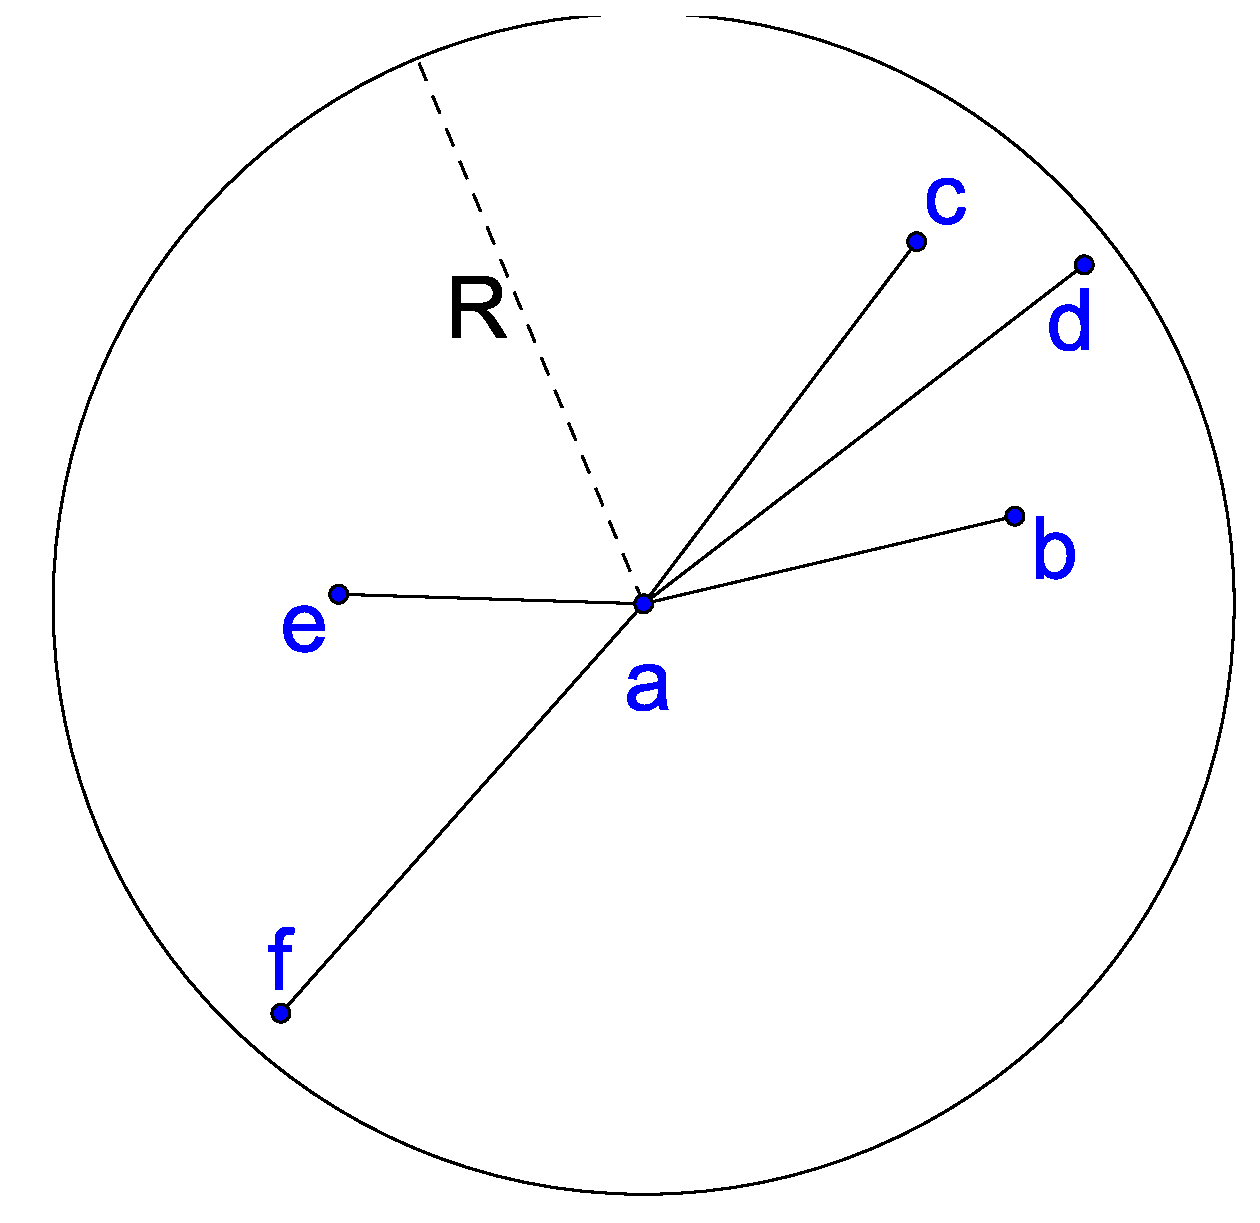
\includegraphics[width=0.5\linewidth]{eps/PDT_1.eps}
\caption{An example graph with unit disk radius $R $ with all edges drawn which are incident on $a $.}
\label{fig:PDT_1}
\end{figure}
Consider the graph in figure \ref{fig:PDT_1}.
We will use it as an example for the application of rPDT.
First, node $a $ sends a RTS and all other nodes set a timer relative to the Euclidean distance to $a $.
Since node $e $ is the closest to $a $ and therefore, there cannot be another node in $disk(a,e) $, its timer fires first and sends a CTS.
$f $ overhears that CTS and checks whether or not $e \in disk(a,f) $.
Since $e \in disk(a,f) $ is indeed true, $af \notin GG $.
However, $af $ is still a PDT edge.
The current angle maximizing node $e $ for edge $af $ ($\angle{aef} $) satisfies the conditions that first, $\bigcirc{aef} $ is empty and second, that $\sin{\angle{aef}} \geq\frac{|af|}{R} $ which means that $\bigcirc{aef} $ does not overlap the unit disk of $a $ and hence, $a $ can decide with only one-hop neighborhood information available that $af \in PDT(U)$.
These steps are visualized in figure \ref{fig:PDT_2}.
\begin{figure}[h!]
\centering
\includegraphics[width=0.5\linewidth]{eps/PDT_2.eps}
\caption{The dashed Gabriel Circle of edge $ae $ and $\bigcirc{aef} $ proof that both edges $ae $ and $af $ are PDT-edges.}
\label{fig:PDT_2}
\end{figure}
The subsequent steps are that $b $ and then $c $ sends a CTS, since both edges are Gabriel edges (refer to figure \ref{fig:PDT_3}).
First, $d $ overhears $b $' CTS, calculates that $b \in disk(a,d) $ and finally that $\bigcirc{abd} $ is empty.
From that point $d $ did not stop its timer yet.
When the CTS from node $c $ arrives at $d $, $\bigcirc{abd} $ is not empty anymore and there cannot be another circle which is empty.
$d $ cancels its timer since it is no PDT neighbor.
Figure \ref{fig:PDT_3} shows also the final edge selection of node $a $ after execution of rPDT.
\begin{figure}[h!]
\centering
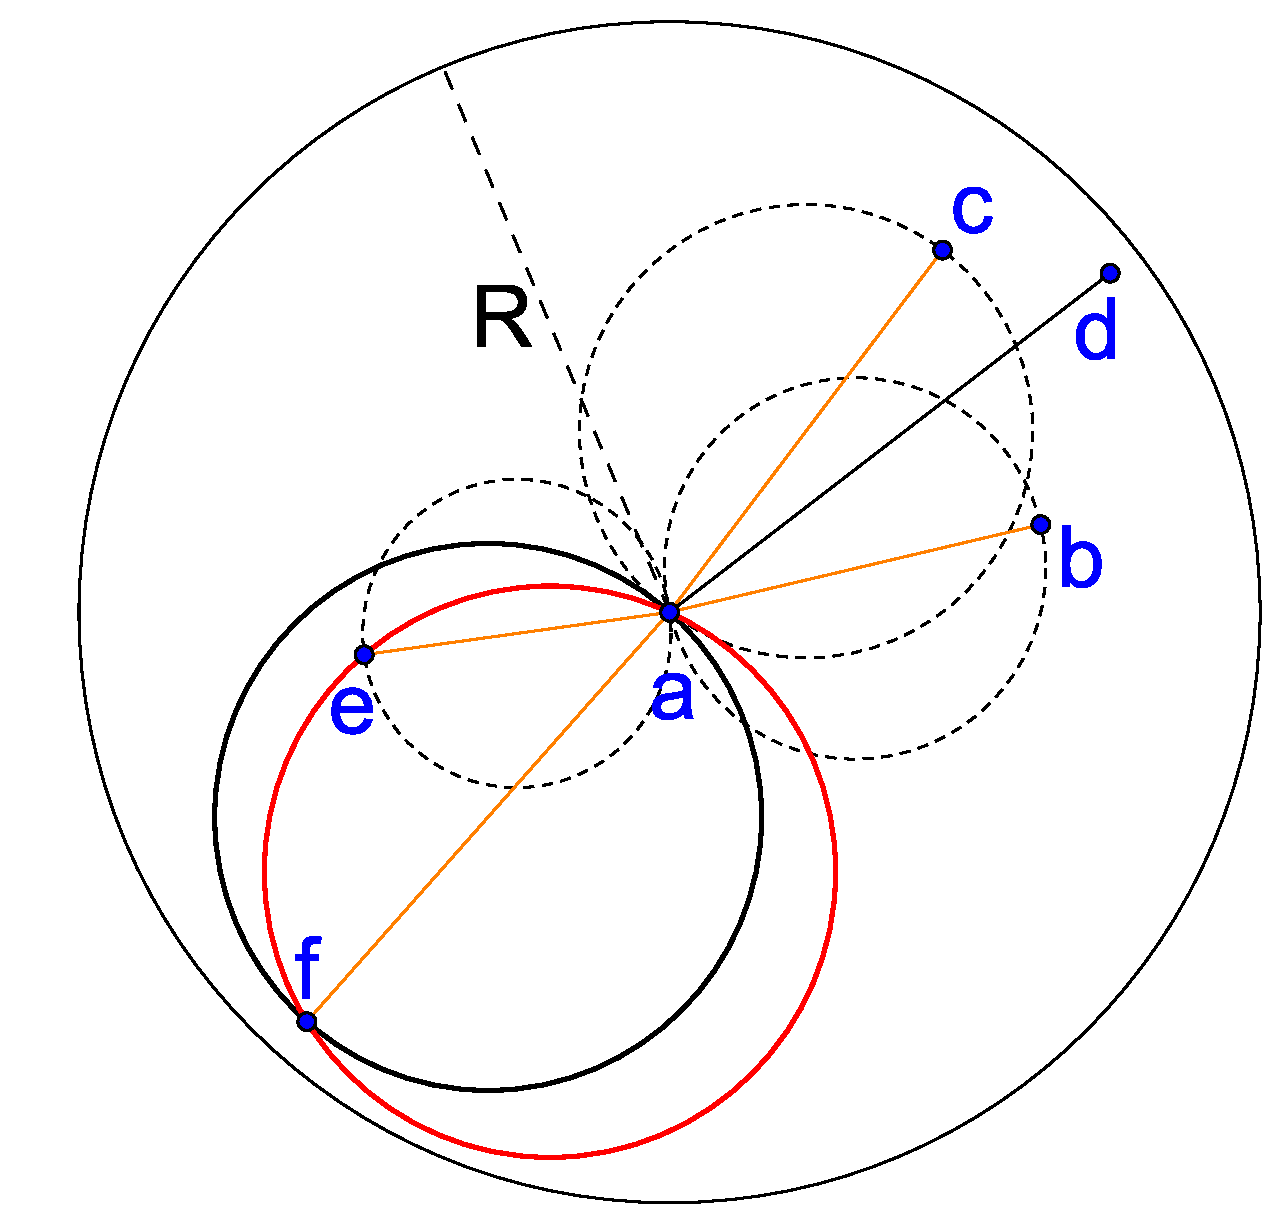
\includegraphics[width=0.5\linewidth]{eps/PDT_3.eps}
\caption{All endpoints of orange edges are PDT neighbors of $a $. Dotted circles are Gabriel circles and the red circle proofs that $af $ is a PDT edge.}
\label{fig:PDT_3}
\end{figure}
%related work: kanj hat neues ergebnis mit knotenbeschränkung kleiner gleich 11...
%improved local algorithms   2012


%reactive planar spanner
%planar spanner with constant node degree
%

%pdt ist äquivalent zum pudel graph -> on the spanning ratio of pdt

%keine fehler passieren,  nachrichten sofort da sind, keine 4 punkte auf kreis, wenn ich sage dass ein punkt eine nachricht zu einem anderen sendet, ist das ein lokaler broadcast   (alle hören mit, und nur der angesprochene reagiert).

%notations und definitions  -> basics foundations
%danach related work 
\section{Related work}

In the past years several topology controls were invented and further developed.
I am interested in local algorithms only, and hence, centralized algorithms are ignored in this related work.
There are a lot of different approaches with different results.
The following is an extract of these approaches and can be divided into two main groups:
\begin{enumerate}
\item reactive algorithms
\item algorithms which produce a planar t-spanner with constant node degree
\end{enumerate}

Reactive algorithms generally need less messages as only localized algorithms to discover the nodes neighbourhoods due to the lack of beaconing.
They do not need the whole $k $-neighbourhood of every node to function, but only a fractional amount of their direct neighbours.
As time of writing there are three reactive algorithms:
\begin{enumerate}
\item Beaconless Forwarder Planarization (BFP)
\item Guaranteed delivery beaconless forwarding (GDBF) with extension
\item reactive Partial Delaunay Triangulation
\end{enumerate}

First, I will describe an algorithm briefly and in the following there is a short section about properties of the produced graph.
The BFP-algorithm (\cite{Ruhrup2010}) is divided into two phases.
First, in the Selection Phase the executing node $F $ starts the algorithm by sending an RTS. 
In the following every node, which receives this message, starts a timer corresponding to a specific delay function.
The closer a node resides to the executing node, the earlier it answers with a CTS. 
If a node $W $ overhears a CTS of a node $W' $ it checks whether or not it is contained in a certain area corresponding to node $W' $ and $F $.
This area is defined by geometric regions, in the following denoted as $Reg(A, B) $, with $A $ and $B $ being two nodes specifying this region.
The minimum region $Reg(F, W') $ is the Gabriel circle $disk(F, W') $ and the maximum region $Reg(F, W') $ is the Relative Neighbourhood Graph lune over $F $ and $W' $.
The latter describes the area of the intersection of two circles around two neighbouring nodes $UV $ with radii equal to $|UV| $ and with middlepoints $U $ and $V $, respectively.
Different regions cause the algorithm to use different amounts of messages.
This will be discussed later.

Suppose $W $ is contained in such an area it cancels its timer and is, henceforth, called a \emph{hidden node}.
Hidden nodes further participate in the algorithm.
If a hidden node $H $ receives a message from another node $T $, it memorizes this node if $H $ lies in the former defined region. 

The Protest Phase lets hidden nodes protest against violating edges.
An edge $UV $ is called a violating edge if there is a node in $Reg(U, V) $.
If hidden nodes have nodes they memorize they restart the above timer.
As soon as a message from another hidden node $W' $ arrives at hidden node $W $, the latter checks its memorized nodes:
A node $X $ can be removed from the set of memorized nodes if $W' \in Reg(F,X) $.
If the timer of a node expires and there are still nodes which are memorized, the node sends a protest message.
The forwarder node $F $ removes violating edges when it receives protests.

This algorithm performed on each node of a graph $G $ produces a planar subgraph $G' $, which can be used for routing algorithms (refer to \cite{Ruhrup2010}).
However, $G' $ is not a t-spanner of $G $ and has no constant node degree despite the underlying region ($GG, RNG, CNG $) (refer to ... for an example of these three regions).

$GDBF $ is a scheme to forward messages in a network.
All messages will be greedy forwarded to the node which lies closest to the destination until a node which has no neighbours closer to the destination, called a local minimum, is reached.
From that point a recovery mode is used until the local minimum is exited and the algorithm can switch back to greedy mode.
In greedy mode the message holder broadcasts a RTS-message to all neighbours.
Every neighbour instantiates a timer with length depending on how far the neighbour is away from the destination. 
Nodes closer to the destination answer earlier.
A CTS-message is sent as soon as the timer expires and the message holder forwards the message to its sender. 
Every other nodes cancels its timer and remain silent.
In recovery mode a RTS message from the message holder is as well sent.
Now, all neighbours instantiate a timer corresponding to the distance to the message holder $M $ (closer nodes respond first).
If a neighbour $N $ overhears another nodes $N' $ message, it cancels its timer if $N' \in disk(M, N) $.
For more detailed information, refer to \cite{Chawla2006}.

GDBF can be extended to reactively produce a planar subgraph 





\section{Algorithm}
This chapter introduces the $reactive Modified Yao Step $ and explains it's functionality.
First, there is the basic version of this algorithm, followed by an improved version which needs less messages to construct a node's neighborhood.
 
\algrenewcommand\algorithmicprocedure{\textbf{}}
\begin{algorithm}\small
\caption{Modified Yao Step}\label{MYS}
\begin{algorithmic}[0]

\Statex \textbf{Input:} planar, t-spanner $G $; integer $k\geq 14 $
\Statex \textbf{Output:} planar, t-spanner $G' $ with constant node degree

\Statex

\For{each node $p\in G $}
	\State Define $k $ disjoint cones of size $2\pi/k $ around $p $.
	\State Select for each non empty cone the shortest edge.
	\For{each maximal sequence $s $ of empty cones}
		\If{$|s|==1 $}
			\State Let $nx $ and $ny $ be the incident edges on $p $ clockwise and \State counterclockwise, respectively, from the emtpy cone.
			\If{either $nx $ or $ny $ has already been selected}
				\State select the other edge
				\Else
				\State Select the shorter edge
			\EndIf 
		\Else
			\State select the first $\lfloor \frac{|s|}{2} \rfloor $ unselected edges incident on $n $ clockwise from $s $
			\State select the first $\lceil \frac{|s|}{2} \rceil $ unselected edges incident on $n $ counterclockwise from $s $
		\EndIf
	\EndFor
\EndFor
\State $ G' $ is the subgraph of $G $ consisting of all nodes which are in $G $ and all edges which fulfil that both endpoints of this edge have selected it. 
\end{algorithmic}
\end{algorithm}





\subsection{Proof of correctness}
\begin{proof}
\begin{equation*}
\begin{split}
	MYS(PDT) &\leftrightarrow RMYS\\
	MYS(PDT(v)) &\stackrel{a)}{\leftrightarrow} rMYS(rPDT(v)) \\
    MYS(PDT(v)) &\stackrel{b)}{\leftrightarrow} rMYS(PDT(v))\\
    MYS(PDT(v)) &\stackrel{c)}{\leftrightarrow} MYS(PDT(v)) 
\end{split}
\end{equation*}
We need to proof that the proposed reactive version of this algorithm is equal to a simple concatenation of first, the Partial Delaunay Triangulation and secondly, the Modified Yao Step on any node $v \in G$.
a) is the fragmentation of the proposition applied to a node $v $.
It is well known that $rPDT $ produces the same graph as the simple local approach, so b) holds true.
$rMYS $ does the same calculation as $MYS $ until the broadcast in the end.
Therefore, we need only to look at this broadcast.
The executing node $v $ sends a broadcast which must be overheard by all $PDT $ -Neighbors of $v $.
Because of the assumptions that every message arrives and arrives instantaneously, the message cannot get lost.
Every informed node sends an answer back which must arrive.
Hence, $v $ can check whether or not each node in it's neighborhood accepts this edge.
This leads to the same behavior MYS does and therefore, c) is true completing this proof.
\end{proof}

\subsection{Message Complexity}
Let $N_{PDT}(u) $ be the message complexity of $PDT $ creating the neighborhood of Node $u \in G$.
First, $rPDT $ needs at most $n $ messages to create the $PDT $-neighborhood.
Next, the executing node sends at most $k $ messages to its neighbors to ask whether they accept their connection.
$k $ answers come back and therefore $k * 2 $.
Every one of this $k $ neighbors needs to calculate it's $PDT $-neighborhood and hence, $k*N_{PDT}(u) $.
The following equation put these reflections into one formula.
\begin{equation*}
\begin{split}
N_{RMYS}(u) &= \underbrace{N_{PDT}(u)}_{\theta (n)} +k *\underbrace{2}_{\theta (1)} + k*\underbrace{N_{PDT}(v)}_{\theta (n)} \\
\theta (N_{RMYS}(u)) &= \theta (n) 
\end{split}
\end{equation*}
Since $k $ is a constant it can be omitted in $O $-Notation.
The sum of the same complexity remains in the same complexity and hence, the complexity of this algorithm is $\theta (n) $.

\subsection{•}

\section{Simulation results}
The simulation was performed in Sinalgo\footnote{http://www.disco.ethz.ch/projects/sinalgo/}.
Sinalgo is a simulation framework which can test and validate network algorithms and at the same time it offers a graphical view on the programmed processes as well as a fast batch mode.

There are two different simulation runs.
The first one calculated the Euclidean and hop spanning ratio of PDT and RMYS and the second one counted the messages which were needed to construct PDT, RMYS and the amount of messages needed by two hop beaconing.
1000 random connected graphs for each node density from 5 to 20 were used.
The numbers of nodes $n $ used for each density were calculated with the following formula:
\begin{equation*}
n =round( \frac{D_x \cdot D_y}{\pi \cdot R^2} \cdot density)
\end{equation*}
Hereby, $D_x=1000 $ and $D_y=1000 $ are the dimension of the simulation plane and $R = 100 $ is the unit disk radius.

\bigskip

The simulations are based on the following assumptions.
\begin{itemize}
\item All nodes are static meaning they cannot move.
\item All calculations are ordered into synchronous rounds. 
At the beginning a node receives all messages sent in the round before.
It follows a general calculation phase and at last a node can send messages.
\item Messages arrive instantaneously and cannot get lost.
Every message which was sent, arrives for sure in the round after it was sent.
\item There are no 4 nodes which are co-circular.
\item All graphs are connected.
\end{itemize}

Figure \ref{fig:RMYS_PDT_SpanningRatio} shows the measured spanning ratio of RMYS and PDT to the unit disk graph with respect to node density.
It is noticeable that both lines seem to be the same line.
For density $5 $ the ratio is approximately $1.30 $ and density 20 has approximately a spanning ratio of $1.38 $.
In between 5 and 20 the curve is increasing slightly and has no outliers.

Since both lines are almost identical it is possibly true that RMYS has also a constant spanning ratio which is a fractional amount greater than the proven spanning ratio of PDT (refer to \cite{Neumann2012} for proof).

\begin{figure}[h!]
\centering
\includegraphics[width=1.0\linewidth]{eps/RMYS_PDT_SpanningRatio.eps}
\caption{Measured Euclidean spanning ratio of Reactive Modified Yao Step (RMYS) and Partial Delaunay Triangulation (PDT) with respect to the unit disk graph in context to the node density. 1000 Simulations per density.}
\label{fig:RMYS_PDT_SpanningRatio}
\end{figure}


Figure \ref{fig:RMYS_PDT_HopSpanningRatio} shows the measured hop spanning ratio of RMYS and PDT to the unit disk graph with respect to node density.
The measured values increase from $3 $ hops at density $5 $ to approximately $4.6 $ at density $20 $.

\begin{figure}[h!]
\centering
\includegraphics[width=1.0\linewidth]{eps/RMYS_PDT_HopSpanningRatio.eps}
\caption{Measured hop spanning ratio of Reactive Modified Yao Step (RMYS) and Partial Delaunay Triangulation (PDT) with respect to the unit disk graph in context to the node density. 1000 Simulations per density.}
\label{fig:RMYS_PDT_HopSpanningRatio}
\end{figure}



In figure \ref{fig:RMYS_PDT_Beaconing_Neighbors.eps} is the message consumption with respect to node density shown.
"PDT on neighbors" shows the amount of messages PDT uses to create the 2 hop PDT neighborhood of one random node within the graph borders and at least unit disk radius $R=100 $ away from the borders to ensure the correct node density.
In this example the amount of messages RMYS and PDT on neighbors uses are almost equal.
The messages used in 2 hop beaconing are much more.
Additionally, the increase from one density to another is greater than the increase in PDT and RMYS.
At density $5 $ beaconing uses almost twice as much messages as RMYS and at density $20 $ it uses almost tenth times as much messages as RMYS.
For reference, the amount of messages which PDT uses to create the 1 hop PDT neighborhood of the same node as above is shown.
Notice that PDT is message optimal (refer to \cite{Benter2013} for proof).

\begin{figure}[h!]
\centering
\includegraphics[width=1.0\linewidth]{eps/RMYS_PDT_Beaconing_Neighbors.eps}
\caption{This plot shows the needed messages to construct the RMYS-neighborhood on a given node with respect to the node density in a 2-hop beaconing approach (Beaconing) and in a reactive way (RMYS). Additionally, the messages rPDT uses to construct the PDT-neighborhood of a node (PDT) and its neighbors (PDT on Neighbors) are shown. 1000 Simulations per density.}
\label{fig:RMYS_PDT_Beaconing_Neighbors.eps}
\end{figure}

Figure \ref{fig:RMYS_PDT_Neighbors} shows the message consumption with respect to node density between RMYS and PDT on neighbors in order to notice the small differences.
In fact RMYS uses always one message more than PDT on neighbors.
For reference, the message consumption for PDT on one node is shown as well.

\begin{figure}[h!]
\centering
\includegraphics[width=1.0\linewidth]{eps/RMYS_PDT_Neighbors.eps}
\caption{The messages needed to construct the PDT-neighborhood of a node (PDT) and its neighbors (PDT on Neighbors) are shown. Additionally, the message usage of the RMYS neighborhood creation is visualized. 1000 Simulations per density.}
\label{fig:RMYS_PDT_Neighbors}
\end{figure}


Refer to figure \ref{fig:RMYS_PDT_avrNeighbors} to see the average and maximal neighbors of the RMYS and the PDT graph.
Density $5 $ leads to approximately $3.6 $ neighbors and almost $6 $ neighbors at density $20 $.
The maximal neighbors differ for both graphs from $6.89 $ at density $5 $ to approximately $10.35 $ for RMYS and $10.44 $ for PDT at density $20 $.
The differences of the maximal neighbors for RMYS and PDT at high densities is explained in REF.

\begin{figure}[h!]
\centering
\includegraphics[width=1.0\linewidth]{eps/RMYS_PDT_avrNeighbors.eps}
\caption{Average and maximal Neighbors of Reactive Modified Yao Step (RMYS) and Partial Delaunay Triangulation (PDT) with respect to node density. 1000 Simulations per density.}
\label{fig:RMYS_PDT_avrNeighbors}
\end{figure}


Figure \ref{fig:RMYS_PDT_UDGNeighborsRatio} shows the amount of neighbors in the subgraphs RMYS and PDT of a random node divided by the amount of neighbors in the unit disk model of the same node.
A value of $1 $ corresponds to all unit disk neighbors are neighbors in the subgraph.
At density $5 $ approximately $0.8 $ percent of all unit disk neighbors are PDT and RMYS neighbors.
At density $20 $ this percentage dropped to $0.33 $.

\begin{figure}[h!]
\centering
\includegraphics[width=1.0\linewidth]{eps/RMYS_PDT_UDGNeighborsRatio.eps}
\caption{The average neighbors for Reactive Modified Yao Step (RMYS) and Partial Delaunay Triangulation (PDT) divided by the average neighbors in the unit disk model are shown. 1000 Simulations per density.}
\label{fig:RMYS_PDT_UDGNeighborsRatio}
\end{figure}

\begin{figure}[h!]
\centering
\includegraphics[width=1.0\linewidth]{eps/RMYS_PDT_MessagesPerNeighbors.eps}
\caption{The messages needed to construct the RMYS neighborhood (RMYS), the PDT neighborhood of a node (PDT) and its neighbors (PDT on Neighbors) divided by the actual neighbors in this subgraph are visualized. 1000 Simulations per density.}
\label{fig:RMYS_PDT_MessagesPerNeighbors}
\end{figure}

In Figure \ref{fig:RMYS_PDT_MessagesPerNeighbors} is the number of used messages by a topology control divided by the obtained neighbors in the specific subgraph visualized.
Here, $1 $ corresponds to for each neighbor in the subgraph $1 $ message was sent.
PDT uses not much more than this.
At density $5 $ PDT sents approximately $1.33$ and at density $20 $ approximately $1.18 $ messages per neighbor.
PDT on neighbors and RMYS send $6.2 $ and $6.5 $, respectively, messages per neighbor at density $5 $.
At density $20 $ PDT on neighbors uses $8.4 $ and RMYS $8.6 $ messages per neighbor.





\section{Notations and Definitions}
In this part of this work we define some notations and declare definitions which we will make use of.
$\bigcirc{ABC} $ is a circle with $A, B, C $ on its border.
The circle with center $O $ is denoted with $(O) $.
$\triangle{ABC} $ is the triangle with corners $A,B $ and $C $.
Furthermore, we assume that there are no four points in any graph which are cocircular.

\subsection{Gabriel Graph}
The Gabriel Graph, denoted as $GG $, is the graph which contains all nodes of a supergraph $U $ and it contains an edge $UV \in U $ if the Gabriel circle of $UV $ contains no other node.
The Gabriel circle of an edge $UV $ is denoted as $disk(U, V) $.
It is the circle with $U $ and $V $ on its border and with its center on line $UV $. 
In this work $U $ is the unit disk graph with unit disk radius $R = 1 $.

\section{Proof}
Let $U $ be the Unit Disk Graph of the Euclidean Graph $E $ with a set of nodes $S $ in the plane as vertex-set and containing edge $AB $ if $|AB| \leq R $ with unit disk radius $R=1 $.
The authors of \cite{kanj} use $LDel^{(2)}(U) $ as the underlying subgraph of the Modified Yao Step.
$LDel^{(2)}(U) $ is defined as the union of the Gabriel-graph and the subgraph of U in which the circumcircle of every triangle does not contain a 2-hop-neighbor of the nodes which create the triangle.
However, it is not known whether $LDel^{(2)}(U) $ can be constructed reactively.
At this point I want to introduce the \emph{Partial Delaunay Triangulation (PDT)} \cite{pdt} which might be a valid replacement.
The following part of this work will examine the possibility of this replacement and, thus, proving the correctness of the following proposition:

\begin{prop}
\label{mastertheorem}
Let $G $ be the PDT-subgraph of $U $.\\
For every integer $k \geq 14 $, there exists a subgraph $G' $ of $G $ such that $G' $ has maximum degree $k $ and stretch factor $1+2\pi (k*\cos{\frac{\pi}{k}})^{-1} $.
\end{prop} 


With $GG $ being the Gabriel Graph, we define the Partial Delaunay Triangulation as follows:
\begin{definition}
\label{pdt-def}
An edge $UV \in U $ is in $G $ if either 
\begin{enumerate}
\renewcommand{\labelenumi}{(\roman{enumi})}
 \item $UV \in GG $
 \item or $\exists{W} \in U : $ maximizes $\angle{UWV} $, $\bigcirc{UVW}  \backslash \{U, V, W\} = \emptyset $ and $\sin{\angle{UWV}} \geq\frac{|CA|}{R} $, with $R>0 $ being the unit disk radius.
\end{enumerate} 
\end{definition}


Additionally, the following Delaunay graph property is being used:
\begin{lemma}
\label{emptyregion}
If CA and CB are edges of the PDT graph then the region $R_1 $ of $(O)=\bigcirc{ABC} $ subtended by chord CA and away from B and the region $R_2 $ of $(O) $ subtended by chord CB and away from A contain no points that are two hop neighbours of A, B and C.
\end{lemma}


Refer to Figure \ref{fig:empty_region} for a graphical illustration of the above lemma.
This property also holds true for PDT.


\begin{proof}
Let $disk(A, C) $ be the circle with $C $ and $A $ on it`s border and the middlepoint on Line $CA $.
Since $CA \in G $ either: 
\begin{enumerate}
\renewcommand{\labelenumi}{(\roman{enumi})}
\item $CA \in GG $:

$B $ cannot lie inside $disk(A, C) $. 
Since $disk(A, C) $ can overlap circle $\bigcirc{ABC} $ on one side of $AC $ only (where $B $ is), $R_1 $ must be completely inside $disk(A, C) $.
\item or $CA \in G\backslash GG $ is satisfied. 

Since $CA \in G $ and $CA \notin GG $, $\exists W\in U : W$ maximizes the interior angle $\angle{CWA}  $, more specifically, $W $ is the closest node to $CA $.
There are two cases, where $W $ can be located:
\begin{enumerate}
\renewcommand{\labelenumi}{(\alph{enumi})}
\item $W $ lies in the halfplane subtended by line $CA $ away from $B $.

$W $ cannot reside in $R_1 $, since the circumcircle $\bigcirc{ACW} $ would contain $B $, which is not allowed by precondition.
Thus, $W \notin R_1 $ is true.
Therefore, $\bigcirc{ACW} $ does certainly contain $R_1 $.

\item $W $ lies in the halfplane subtended by line $CA $ towards $B $.

Since $W $ is the angle maximizing node with respect to $CA $, the following is true: $\angle{CWA} \geq \angle{BCA} $.
Therefore, $W \in \bigcirc{ABC} $ and since $\bigcirc{ACW} $ does not overlap $\bigcirc{ABC} $ on the side subtended by line $CA $ where $W $ is, it must overlap $\bigcirc{ABC} $ on the other side.
Thus, it must contain $R_1 $ completely.

\end{enumerate} 


\end{enumerate}
These deductions work for $R_2 $ analogously.
Therefore, $R_1 $ and $R_2 $ cannot contain one or two hop neighbours of $A $, $B $ and $C $. 


\end{proof} 



We need to show that there is a path from $A $ to $B $.
First, we divide the proof into two cases: when $\triangle{ABC} $ contains nodes of G and when this triangle is devoid of any nodes of G.
%Preliminaries
\begin{figure}[h!]
\centering
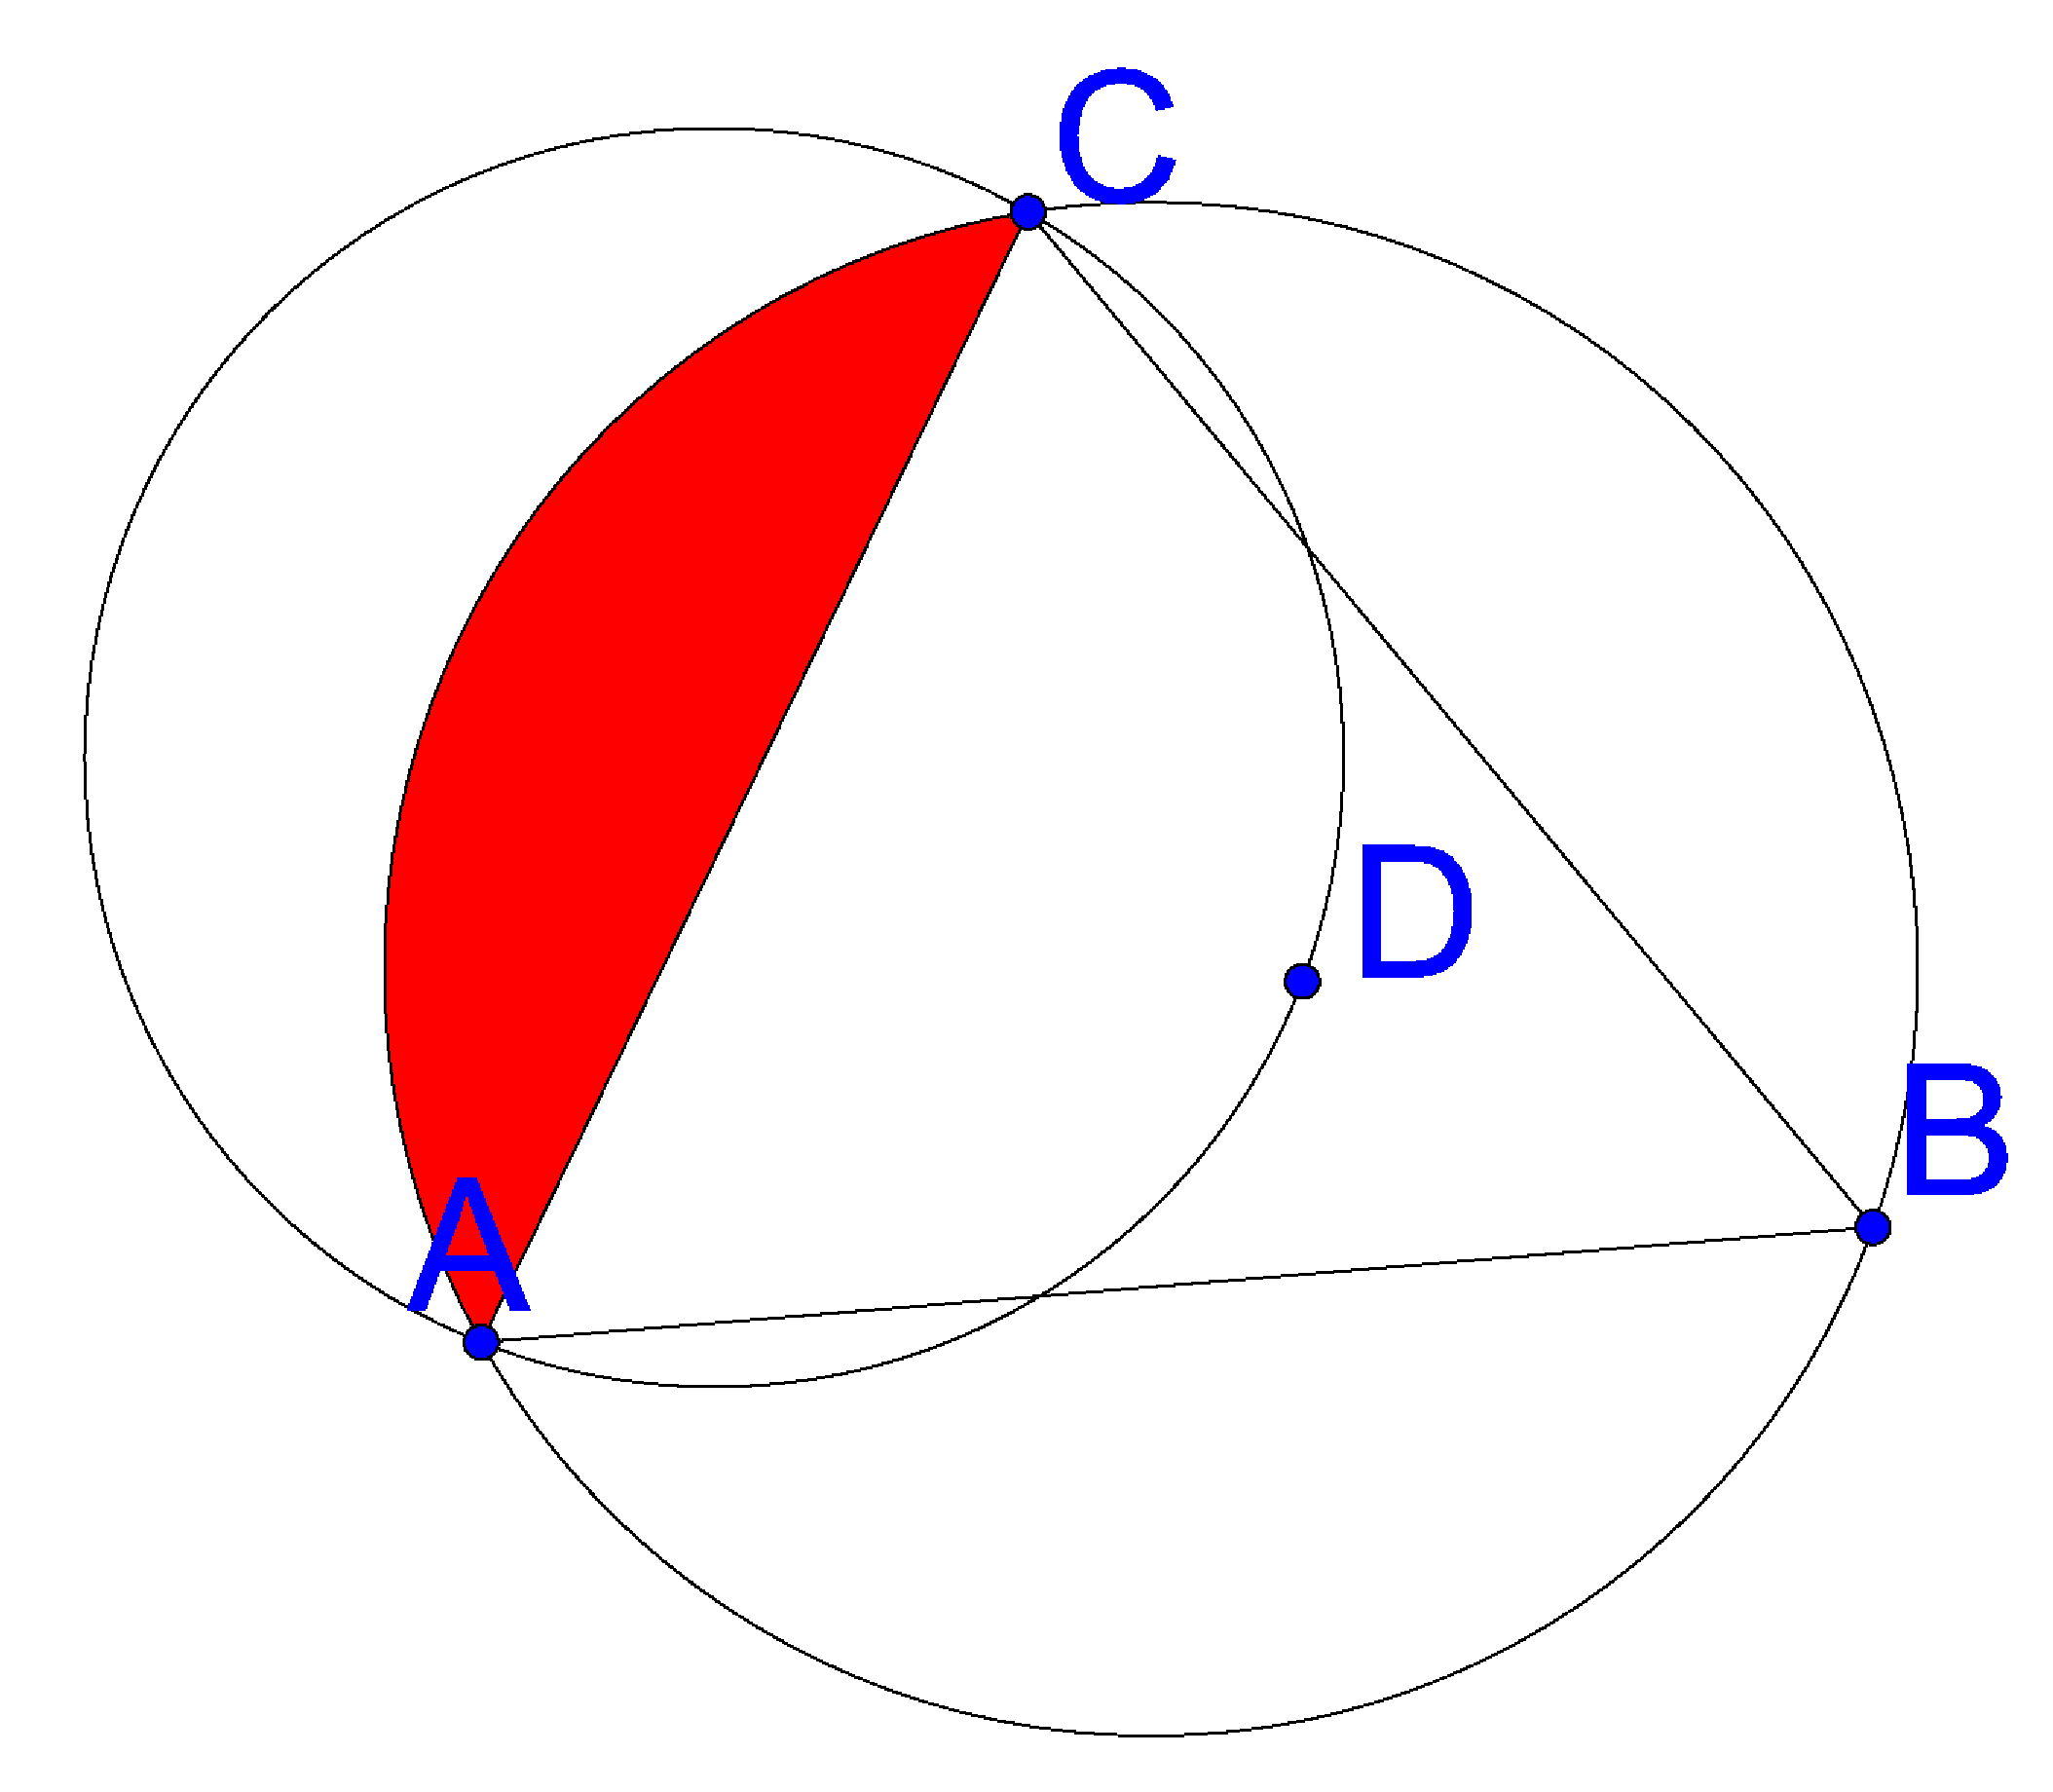
\includegraphics[width=0.2\linewidth]{eps/noPointinRegion.eps}
\caption{The red marked region contains no Points of G because it is always contained in $\bigcirc{ACD} $ which must be empty by definition.}
\label{fig:empty_region}
\end{figure}

Keil and Gutwin \cite{keil} proved the existence of a path between the points $A $ and $B $ and showed that the length of this path is delimited by the length of the arc from $A $ to $B $ on the circle $\bigcirc{ABC} $.
This path connects $A $ and $B $ when no other points of G are inside $\triangle{ABC} $.
The only precondition is that lemma \ref{emptyregion} holds (which it does).
This path is called the \emph{outward path}.
 
First, notice the recursive definition of this path taken from \cite{kanj}:
\begin{enumerate}
\item \textbf{Base case:} If $AB \in G $, the path consists of edge AB.
\item \textbf{Recursive step:} Otherwise, a point must reside in the region $R_3 $ of $(O) $ subtended by chord AB and away from C. 
Let $T $ be such a point with the property that the region of $\bigcirc{ATB} $ subtended by chord $AB $ closer to $T $ is empty. 
We call T an \emph{intermediate point} with respect to the pair of points $(A, B) $.
Let $(O_1) $ be the circle passing through $A $ and $T $ whose center $O_1 $ lies on segment $AO $  and let $(O_2) $ be the circle passing through $B $ and $T $ whose center $O_2 $ lies on segment $BO $.
Then both $(O_1) $ and $(O_2) $ lie inside $(O) $, and $\angle{AO_1T} $ and $\angle{TO_2B} $ are both less than $\angle{AOB} \leq \frac{4\pi}{k} $.
Moreover, the region of $(O_1) $ subtended by chord $BT $ and containing $O_2 $ is empty. Therefore, we can recursively construct a path from $A $ to $T $ and a path from $T $ to $B $, and then concatenate them to obtain a path from A to B.  
\end{enumerate}
Figure \ref{fig:intermediate_point} contains an example for an intermediate point.

The recursive steps assumes $AB \notin G $ and concludes that there must be a point in $R_3 $.
For $G=PDT $ the following lemma proofs the correctness of this assumption:
\begin{lemma}
\label{recursive_step}
For three points $A, B, C \in G $ and $\gamma=\angle{ACB}\leq \frac{2\pi}{k} $ with $k\geq 14 $, $|AB|\leq R $ is satisfied.
\end{lemma} 
\begin{proof}

\begin{equation*}
\begin{split}
  |AB|² &=|BC|²+|AC|² - 2|BC||AC|\cos{\gamma} \\
  &\leq R²+R²   - 2R²\cos{\gamma} \\
  &\leq 2R² - 2R²\cos{\frac{2\pi}{k}}\\
  &\stackrel{a)}{\leq} 2R² - 2R²\cos{\frac{\pi}{7}}\\
  &\stackrel{b)}{\leq} 2R² - 2R²\cdot 0.9 = 0.2R²=\\
  |AB| &\leq \sqrt{0.2} R \leq R
\end{split}
\end{equation*}
In order to minimize $2R²\cos{\frac{2\pi}{k}} $, $\gamma $ must be maximized and hence, it is $\frac{2\pi}{k} $ obtaining a).
Then adjust $\frac{\pi}{7} $ downward to $0.9 $ and receive b).
 
\end{proof}

Lemma \ref{emptyregion} and lemma \ref{recursive_step} proof that there must be a node in $R_3 $, if $AB \notin G $.



\begin{figure}[h!]
\centering
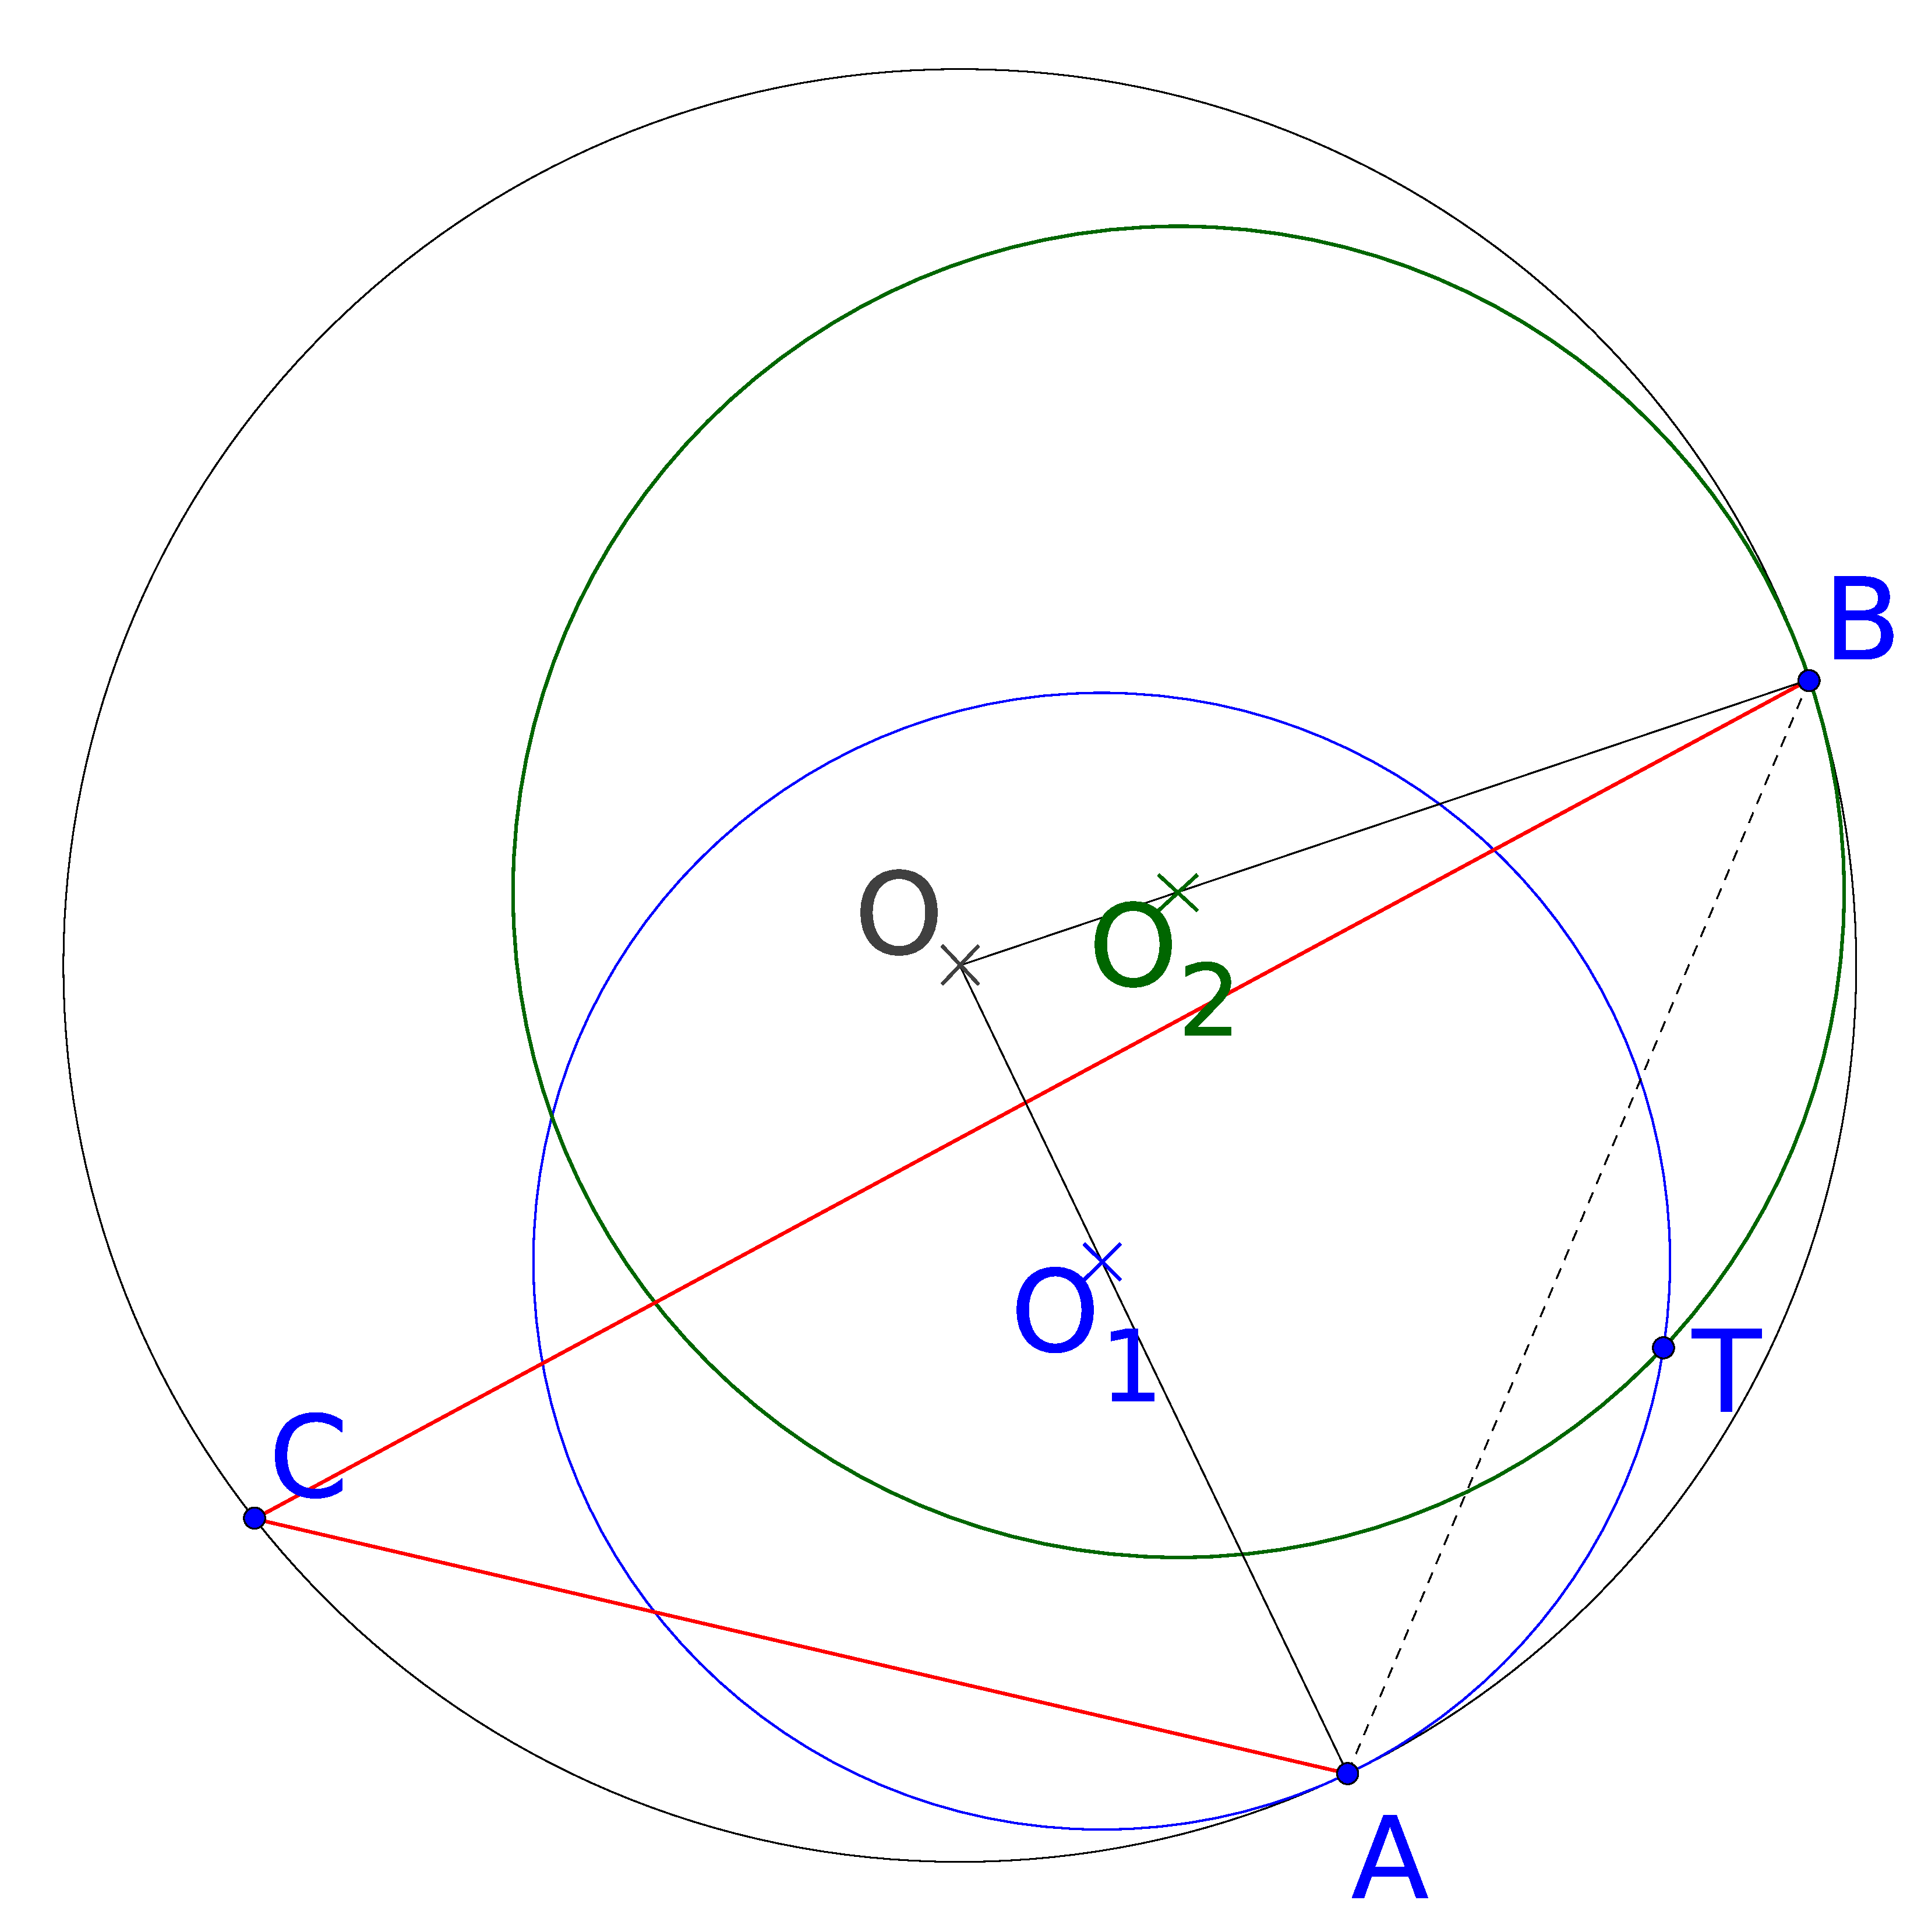
\includegraphics[width=0.5\linewidth]{eps/IntermediatePoint.eps}
\caption{The intermediate point $T $ with respect to pair $(A,B) $, and the circles $O_1 $ and $O_2 $, which are completely within $O $. }
\label{fig:intermediate_point}
\end{figure}


In order to proof proposition \ref{mastertheorem} we need the following proposition (which is from \cite{kanj}):

\begin{prop}
\label{outward_path}
In every recursive step of the outward path construction described above, if $M_p $ is an intermediate point with respect to a pair of points $(M_i, M_j) $, then:
\begin{enumerate}
\renewcommand{\labelenumi}{\alph{enumi})}
\item there is a circle passing through C and $M_p $ that contains no point of G, and
\item circles $\bigcirc{CM_iM_p} $ and $\bigcirc{CM_jM_p} $ contain no points of G, except, possibly, in the region subtended by chords $M_iM_p $ and $M_pM_j $, respectively, away from C.
\end{enumerate}
\end{prop}

\begin{figure}[h!]
\centering
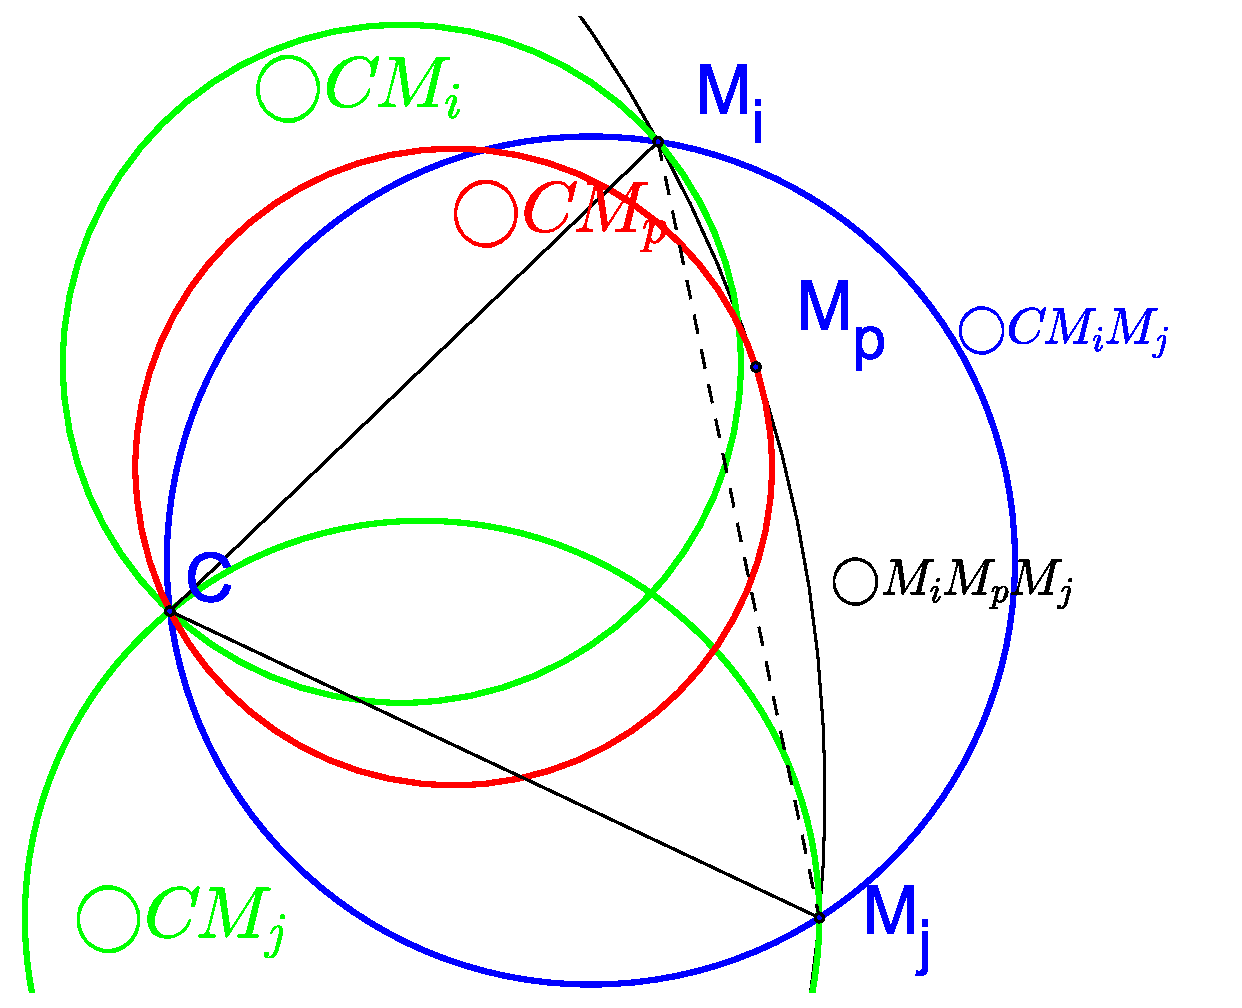
\includegraphics[width=0.9\linewidth]{eps/beweis_outward.eps}
\caption{Example for proof of proposition \ref{outward_path}.}
\label{fig:outward_path_beweis}
\end{figure}

Note that every point $p=1, \cdots, r-1 $, is an intermediate point with respect to a pair $(M_i, M_j) $, where $0\leq i < p <j \leq r  $.
Furthermore, Keil and Gutwin \cite{keil} showed that the length of the path $A =M_0, M_1, \cdots, M_r=B $ is bounded by the length of arc $\overarc{AB} $.
For completeness I copy the proof for proposition \ref{outward_path} from \cite{kanj} with adapted notation.
\begin{proof}

We assume, by induction, that there are circles $\bigcirc{CM_i} $ and $\bigcirc{CM_j} $ passing through $C $ and $M_i $, and $C $ and $M_j $, respectively, containing no points of $G $, and that the circle $\bigcirc{CM_iM_j} $ contains no point of $G $ in the interior of the region $R' $ subtended by chord $M_iM_j $ closer to $C $.
(This is certainly true in the base case because $CA, CB \in G $, by lemma \ref{emptyregion} and by our initial assumptions).

Since $M_iM_j $ is not an edge in $G $, the point $M_p $ chosen in the construction is the point with the property that the region $R $ of $\bigcirc{M_iM_pM_j} $ subtended by chord $M_iM_j $ away from $C $, contains no point of $G $. 
Then the circle passing through $C $ and $M_p $ and tangent to $\bigcirc{M_iM_pM_j} $ at $M_p $ is completely inside $\bigcirc{M_i} \cup \bigcirc{M_j} \cup R \cup R' $, and therefore devoid of points of $G $.
This proves part a).

The region of $\bigcirc{CM_iM_p} $ subtended by chord $M_iM_p $ and containing $C $ is inside $ \bigcirc{M_i} \cup R \cup R' $, and therefore contains no point of $G $ in its interior.
The same is true for the region of $\bigcirc{CM_jM_p} $ subtended by chord $M_jM_p $ and containing $C $, and part b) holds as well.


%Let $G $ be the set of nodes which is created by PDT. 
%Since $CA $ and $CB $ are edges in $G $ there are circles $\bigcirc{CM_i} $ and $\bigcirc{CM_j} $ which have $C $ and $M_i $, and $C $ and $M_j $, respectively, on it's border and do not contain any other nodes of $G $. 
%At this point I assume, without loss of generality, that $M_i $ and $M_j $ lie on the y-axis of the coordinate system and $C $ lies to the left of these points.
%First, notice that $\triangle{CM_iM_j} $ is empty by precondition and the area $R_{\bigcirc{M_iM_pM_j}} $ of $\bigcirc{M_iM_pM_j} $ subtended by chord $M_iM_j $ away from $C $ contains no other points either.
%This proof is divided into three cases.
%\begin{enumerate}
%\item $\bigcirc{CM_p} $ is tangential to $\bigcirc{CM_iM_j} $ at C.
%\item $\bigcirc{CM_p} $ overlaps $\bigcirc{CM_iM_j} $ in the upper halfplane subtended by chord $CM_i $ (away from $M_j $).
%\item $\bigcirc{CM_p} $ overlaps $\bigcirc{CM_iM_j} $ in the lower halfplane subtended by chord $CM_j $ (away from $M_i $).
%\end{enumerate}
%Since the two circles $\bigcirc{CM_p} $ and $\bigcirc{CM_iM_j} $ share the point $C $, $\bigcirc{CM_p} $ cannot overlap $\bigcirc{CM_iM_j} $ on both sides of the edge $CM_p $.
%For case 1 $\bigcirc{CM_p} $ is completely inside $\bigcirc{CM_iM_j} $ and therefore devoid of any points.
%For case 2 $\bigcirc{CM_p} $ is completely inside the area $R_{\bigcirc{M_iM_pM_j}} \cup \bigcirc{CM_iM_j} \bigcirc{CM_i} $ and, therefore, empty.
%$\bigcirc{CM_p} $ cannot overlap $\bigcirc{CM_i} $ because of the following lemma.
%\begin{lemma}
%\label{circles}
%If $A $ and $B $ are points in the plane and are located in different halfplanes of a line $CM_i $, and $A $ and $B $ are not allowed to reside inside a circle $\bigcirc{CM_i} $, there is no circle $\bigcirc{ABC} $ which does not contain $M_i $ and overlaps circle $\bigcirc{CM_i} $.
%\end{lemma}
%\begin{proof}
% Let, without loss of generality, $C $ and $M_i $ be on a line $CM_i $ which is parallel to the y-axis.
%$A $ and $B $ are then located to the left and right of this line.
%You can see this construction in figure \ref{fig:beweis_circles}.
%
%This proof uses a contradiction. % widerspruchsbeweis  -> Florentin fragen
%$A $ cannot reside inside $\bigcirc{CM_i} $, since $CM_i $ is a PDT-edge.
%The circle $c_1 $ must not contain $M_i $ and, therefore, must cross the circle $\bigcirc{CM_i} $ in front of $M_i $.
%Notice that the next part of the circle $c_1 $ must be inside of circle $\bigcirc{CM_i} $, since we started outside.
%Because $c_1 $ must cross $B $ and $B $ lies outside of $\bigcirc{CM_i} $, $c_1 $ crosses a second time $\bigcirc{CM_i} $.
%And the last conclusion is that $C $ is a common point of $\bigcirc{CM_i} $ and $c_1 $.
%Hence, we have got three intersections of $\bigcirc{CM_i} $ and $c_1 $ at least.
%Since $A $ and $B $ lie outside of $\bigcirc{CM_i} $, these two circles are not equal.
%But two circles which intersect at least three times and are not equal, do not exist.
%\end{proof}
%The proof of case 3 works analogously.
%These conclusions proof part a) of proposition \ref{outward_path}.
%
%The following part of this work proofs part b) of the same proposition.
%The main argument of this proof is that $\bigcirc{CM_iM_p} $ is contained completely in the area $\bigcirc{CM_i} \cup  R_{\bigcirc{M_iM_pM_j}} \cup R2_{\bigcirc{CM_iM_j}} $ with $R2_{\bigcirc{CM_iM_j}} $ being the area of $\bigcirc{CM_iM_j} $ subtended by chord $M_iM_j $ closer to $C $.
%I show that every possible position of $\bigcirc{CM_i} $ includes the area $R3_{\bigcirc{CM_iM_p}} $ of $\bigcirc{CM_iM_p} $ subtended by chord $CM_i $ away from $M_j $.
%The proof is divided into three cases of how $\bigcirc{CM_i} $ can be located:
%\begin{enumerate}
%\item $\bigcirc{CM_i} $ is equal to $\bigcirc{CM_iM_p} $.
%\item $\bigcirc{CM_i} $ overlaps $\bigcirc{CM_iM_p} $ in the halfplane subtended from line $CM_i $ away from $M_j $.
%\item $\bigcirc{CM_i} $ overlaps $\bigcirc{CM_iM_p} $ in the halfplane subtended from line $CM_i $ closer to $M_j $.
%\end{enumerate}
%First, assume, without loss of generality, that $C $ and $M_i $ lie on a horizontal line and $M_j $ is located below this line.
%$\bigcirc{CM_iM_p} $ can only overlap $\bigcirc{CM_i} $ on one side of line $CM_i $, since they share these two points.
%
%For case 1, since $\bigcirc{CM_i} $ is empty, $\bigcirc{CM_iM_p} $ must be empty, too.
%
%For case 2, $\bigcirc{CM_i} $ moves up, away from $M_j $, expanding the area in the same direction of which $R3_{\bigcirc{CM_iM_p}} $ is located.
%So, $R3_{\bigcirc{CM_iM_p}} $ cannot overlap $\bigcirc{CM_i} $ in this case.
%
%Case 3, the only case where $R3_{\bigcirc{CM_iM_p}} $ would overlap $\bigcirc{CM_i} $, cannot occur, since $M_p \in G $ and $M_p $ is, obviously, located on $\bigcirc{CM_iM_p} $.
%So, if $\bigcirc{CM_i} $ moves down, towards $M_j $, it would contain $M_p $, which cannot happen, since $\bigcirc{CM_i} $ is a PDT-circle. 
%
%Notice that the proof for $\bigcirc{CM_jM_p} $ works analogously substituting $M_i $ with $M_j $ and vice versa.
 
\end{proof}
\begin{figure}[h!]
\centering
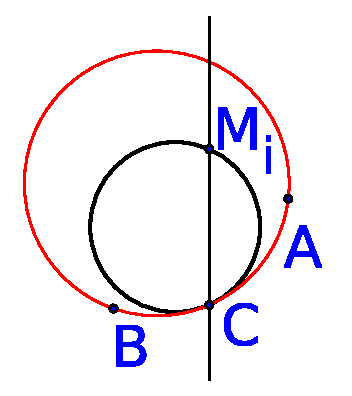
\includegraphics[width=0.5\linewidth]{eps/beweis_circles.eps}
\caption{Example of the construction of lemma \ref{circles}.}
\label{fig:beweis_circles}
\end{figure}
Another fact we need in order to proof proposition \ref{mastertheorem} is the following:
\begin{fact}
\label{outward_3}
If four points $A $, $B $, $C $ and $M_1 $ are on one circle and $C $ and $M_1 $ are on different halfplanes of chord $AB $, then $\angle{AM_1B} + \angle{ACB} =\pi $ is true (please refer to figure \ref{fig:winkel_fuer_outward_3} for an graphical illustration of this lemma).\footnote{see Euklid, book 3, proposition 22, for proof}
\end{fact}

\begin{figure}[h!]
\centering
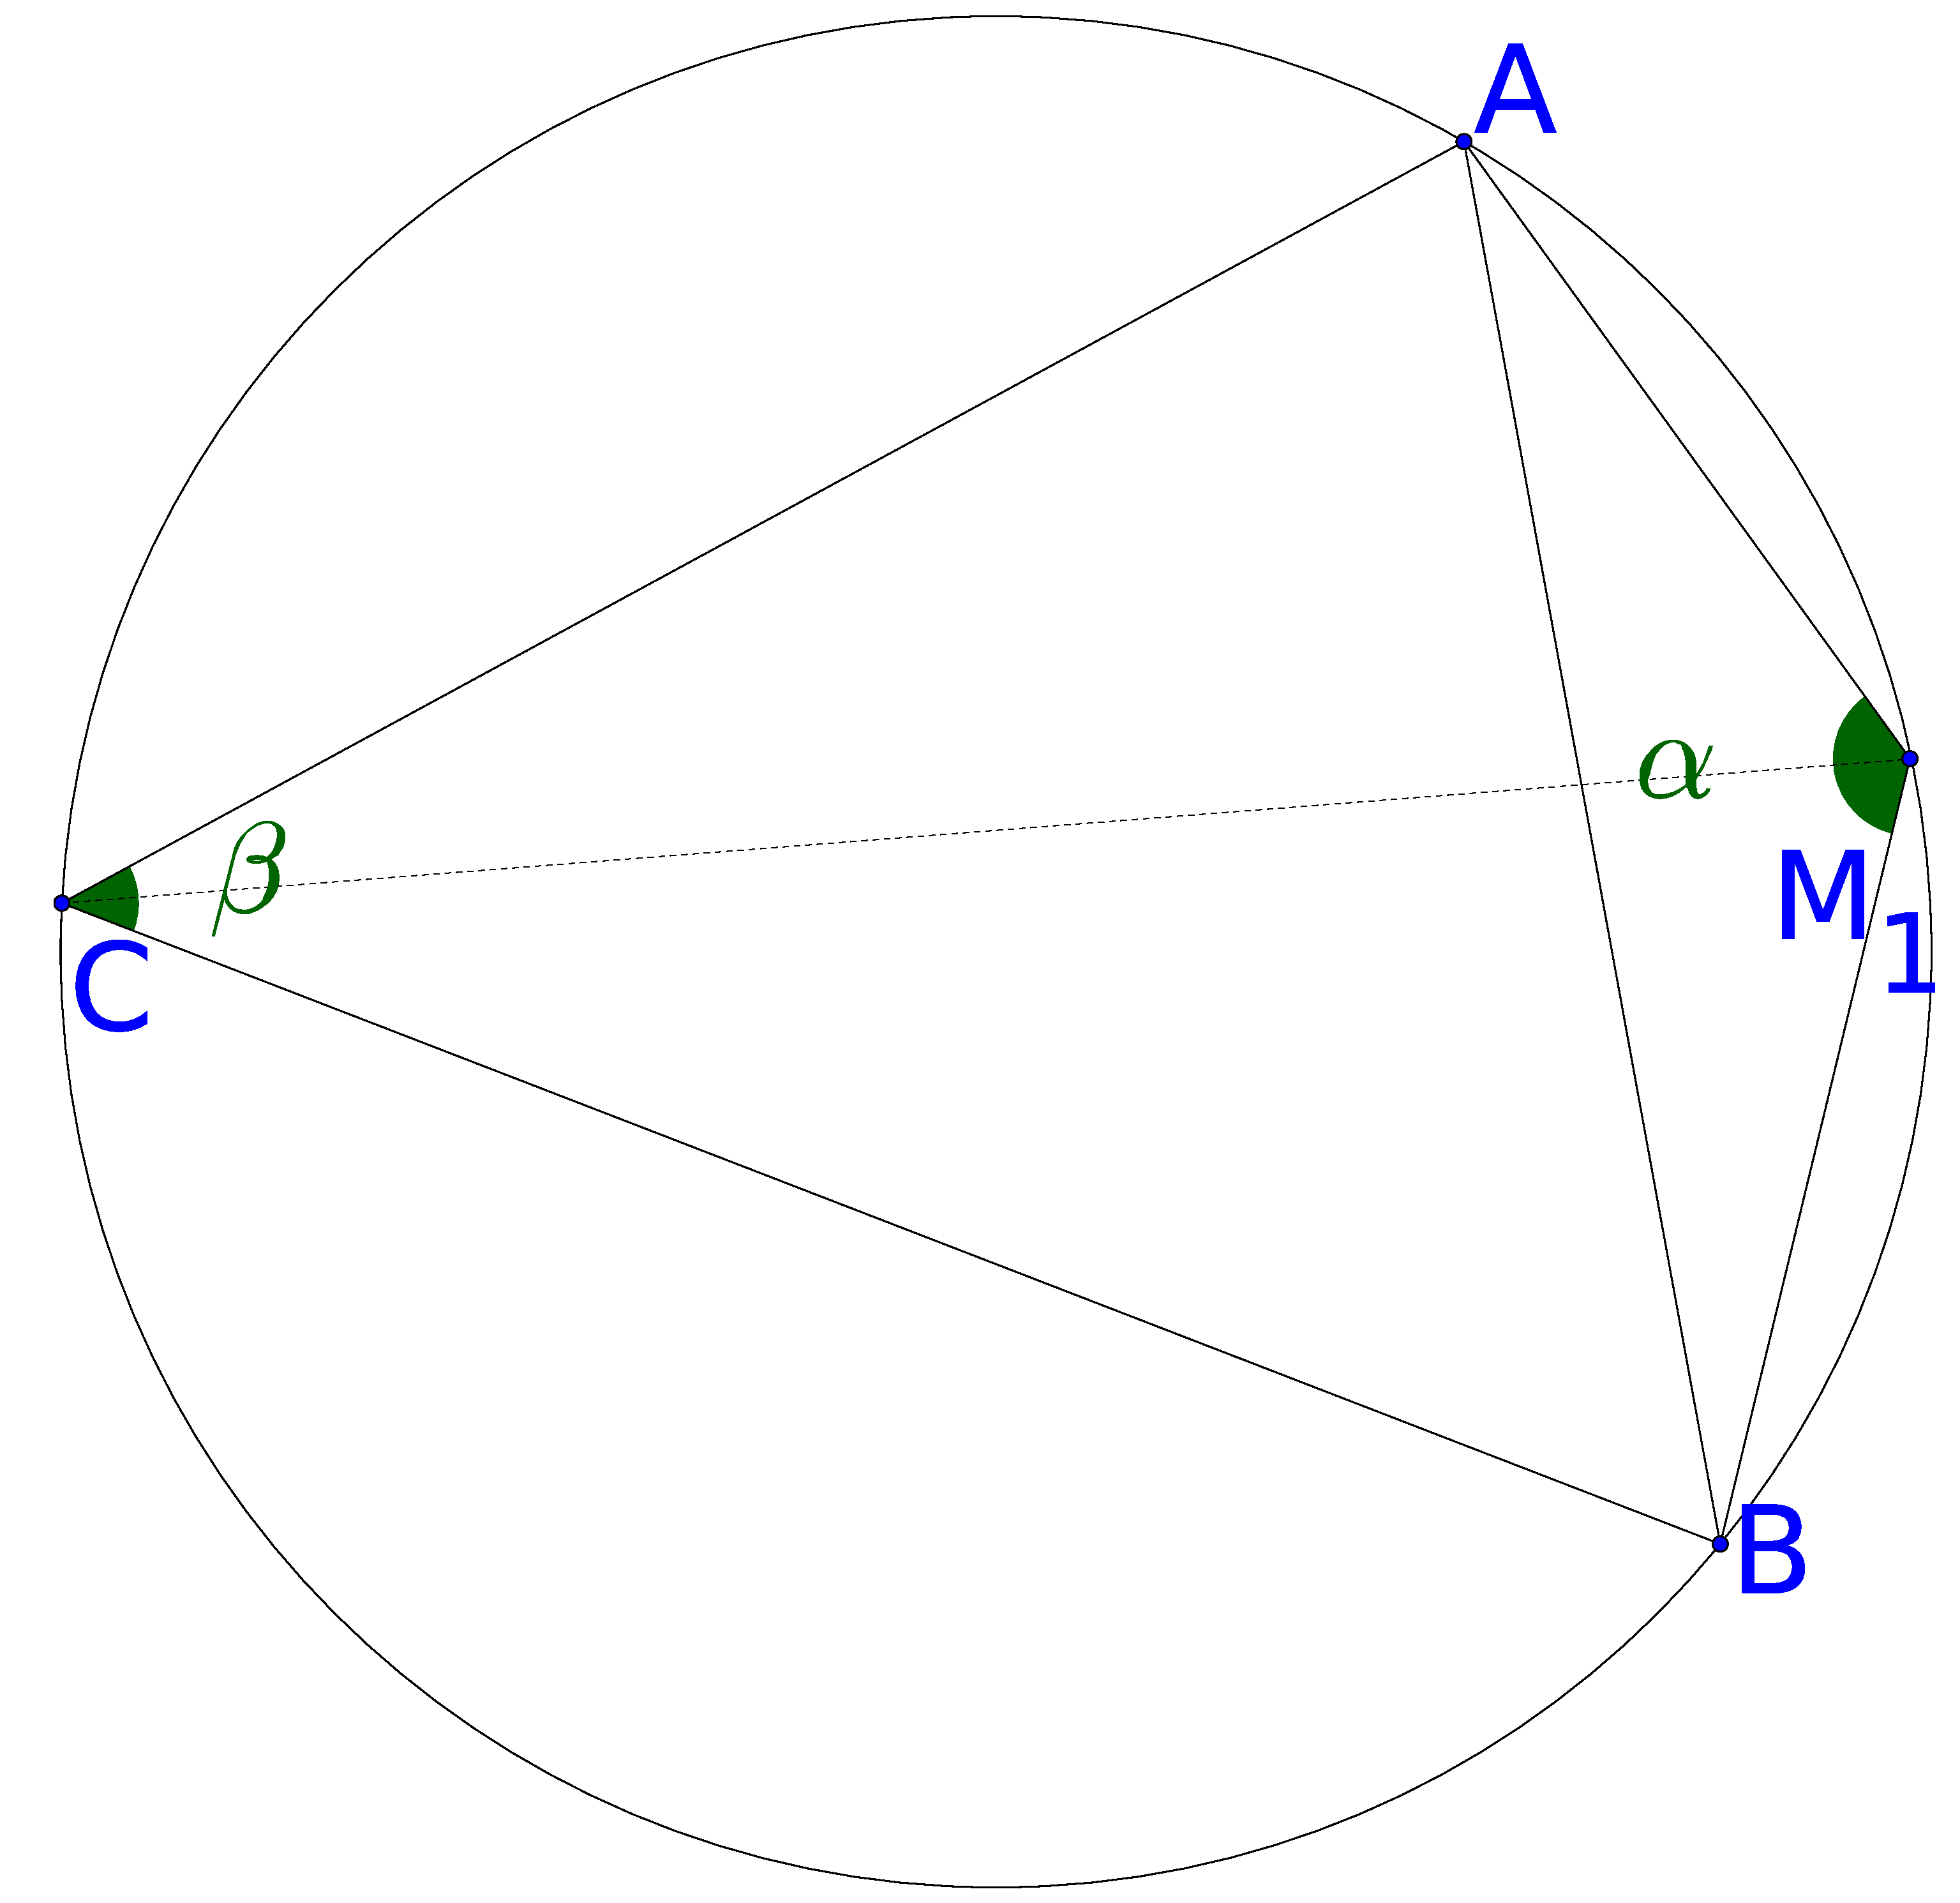
\includegraphics[width=0.4\linewidth]{eps/Winkel_fuer_outward_3.eps}
\caption{Example for lemma \ref{outward_3} }
\label{fig:winkel_fuer_outward_3}
\end{figure}

Now, we can proof the following lemma from \cite{kanj}, which shows, that for the case of the outward path, proposition \ref{mastertheorem} is satisfied:

\begin{lemma}
Let $k \geq 14$ be an integer, and let $CA $ and $CB $ be edges in $G $ such that $\angle{BCA} \leq \frac{2\pi}{k} $ and $CA $ is the shortest edge in the angular sector $\angle{BCA} $. There exists a path $p : A=M_0, M_1, \dotsc, M_r=B $ in $G $ such that:
\begin{enumerate}
\renewcommand{\labelenumi}{(\roman{enumi})}
\item $|CA| + \sum_{i=0}^{r-1}|M_iM_{i+1}| \leq (1+2\pi(k \cos(\frac{\pi}{k}))^{-1})|CB|$
\item There is no edge in $G $ between any pair $M_i $ and $M_j $ lying in the closed region delimited by $CA, CB $ and the edges of $p $, for any $i $ and $j $ satisfying $0 \leq i < j -1 \leq r $.
\item $\angle{M_{i-1}M_iM_{i+1}} > \pi - \frac{2\pi}{k} $, for $i=1,\dotsc,r-1 $.
\item $\angle{CAM_1} \geq \frac{\pi}{2} - \frac{pi}{k} $.
\end{enumerate}	 
\end{lemma}

\begin{proof}
This proof is performed almost equal to \cite{kanj}, but covering more details.
%and $\sin{\theta} = \frac{|AB|}{2|OA|}) $
\renewcommand{\labelenumi}{(\roman{enumi})}%
\begin{enumerate}
\item 
\begin{equation*}
\begin{split}
|CA|+|\overarc{AB}| &= |CB| + 2\theta \cdot |OA| \\
&\stackrel{a)}{=}|CB| + (\frac{\theta}{\sin{\theta}})\cdot |AB| \\
&\stackrel{b)}{=} |CB| + (\frac{\theta}{\cos{\frac{\theta}{2}}}) \cdot |CB|\\
&\stackrel{c)}{\leq} (1+2\pi(k \cos{\frac{\pi}{k}})^{-1}) |CB|  
\end{split}
\end{equation*}
In \cite{keil} Keil and Gutwin proved that the length of the path between $A $ and $B $ is bounded by $|\overarc{AB}|$ and thus, it suffices to show that $|CA| + |\overarc{AB}|\leq (1+2\pi(k \cos{\frac{\pi}{k}})^{-1})$.
Since $|CA| \leq |CB| $, $|CA|+|\overarc{AB}| $ is largest, when $CA $ and $CB $ are symmetrical to the diameter of $\bigcirc{ABC} $, we can assume $|CA|=|CB| $.
$|\overarc{AB}| $ can be replaced with $2\theta \cdot |OA| $ (angle times radius).
For every chord $s $ of a circle $(c) $ it is true, that $s=2r\sin{\frac{\alpha}{2}} $, with $r $ being the radius of $(c) $ and $\alpha $ being the angle between the endpoints of $s $ in middlepoint $c $ facing $s $.
Note that $\alpha = 2\theta $. 
These equations proof a).

Next, substitute $|AB| $ with $|AB| = \sin{\frac{\theta}{2}} \cdot 2|CB| $ and replace $\sin{\theta} $ with the trigonometry identity $\sin{\theta}=2\sin{\frac{\theta}{2}} \cos{\frac{\theta}{2}} $.
You receive equation b).

At last, substitute $\theta $ using inequality $\theta \leq \frac{2\pi}{k} $ with $k > 2 $, obtaining c).

\item  Suppose, $M_i $ and $M_j $ is an edge in $G $, then there exists a circle with these two points on it's border which does not contain any other node of $G $.
So, $M_p $ must lie outside of this circle.
By proposition \ref{outward_path} part a) there is a circle $\bigcirc{CM_p} $ trough $C $ and $M_p $ which is empty.
These two last observations contradict each other, since $\bigcirc{M_iM_j} $ would always contain $M_p $.
If $M_p $ does not reside in the circle $\bigcirc{M_iM_j} $, this circle and the circle $\bigcirc{CM_p} $ would cross at least three times (and are not equal), which cannot exist.

\item Since the angles $\alpha $ and $\beta $ between opposite points of a chord in a rectangle which corners lie on a circle are supplementary, this is a fact: $\angle{AM_1B}=\pi - \angle{ACB} $ (see lemma \ref{outward_3} for more details).
The angle $\angle{M_{i-1}CM_{i+1}} $ is smallest, if $M_{i-1} $ and $M_{i+1} $ lie on the circle. 
Note, by precondition we assume $\angle{BCA} \leq \frac{2\pi}{k} $.
These facts proof following inequalities:
\begin{equation*}
\begin{split}
 \angle{M_{i-1}M_iM_{i+1}}&\geq \pi - \angle{M_{i-1}CM_{i+1}}\\
 &\geq \pi - \angle{BCA} \\ &\geq \pi - \frac{2\pi}{k}\\
\end{split}
\end{equation*}



 %http://www.regentsprep.org/regents/math/geometry/gp15/circleangles.htm
\item Since $M_1 $ is inside the area subtended by chord $AB $ from $\bigcirc{ABC} $ \emph{away} from $C $, it is true that $\angle{CAM_1} \geq \angle{CAB} \geq \frac{\pi}{2} -\frac{\pi}{k} $.
The last inequality is true because:
 \begin{equation*}
  \begin{split}
   \angle{CAB}+\angle{ABC}+\underbrace{\angle{BCA}}_{\leq \frac{2\pi}{k}}&=\pi\\
   \angle{CAB}+\angle{ABC} &\geq \pi - \frac{2\pi}{k} \\
   \angle{CAB} &\geq \frac{\pi-\frac{2\pi}{k}}{2}=\frac{\pi}{2}-\frac{\pi}{k}
   \end{split} 
\end{equation*}
Since $CA \leq CB $, $\angle{CAB} $ can be at most the half of $\pi - \frac{2\pi}{k} $, proving the last inequality.

\end{enumerate}
\end{proof}

 
%\begin{figure}[h!]
%\centering
%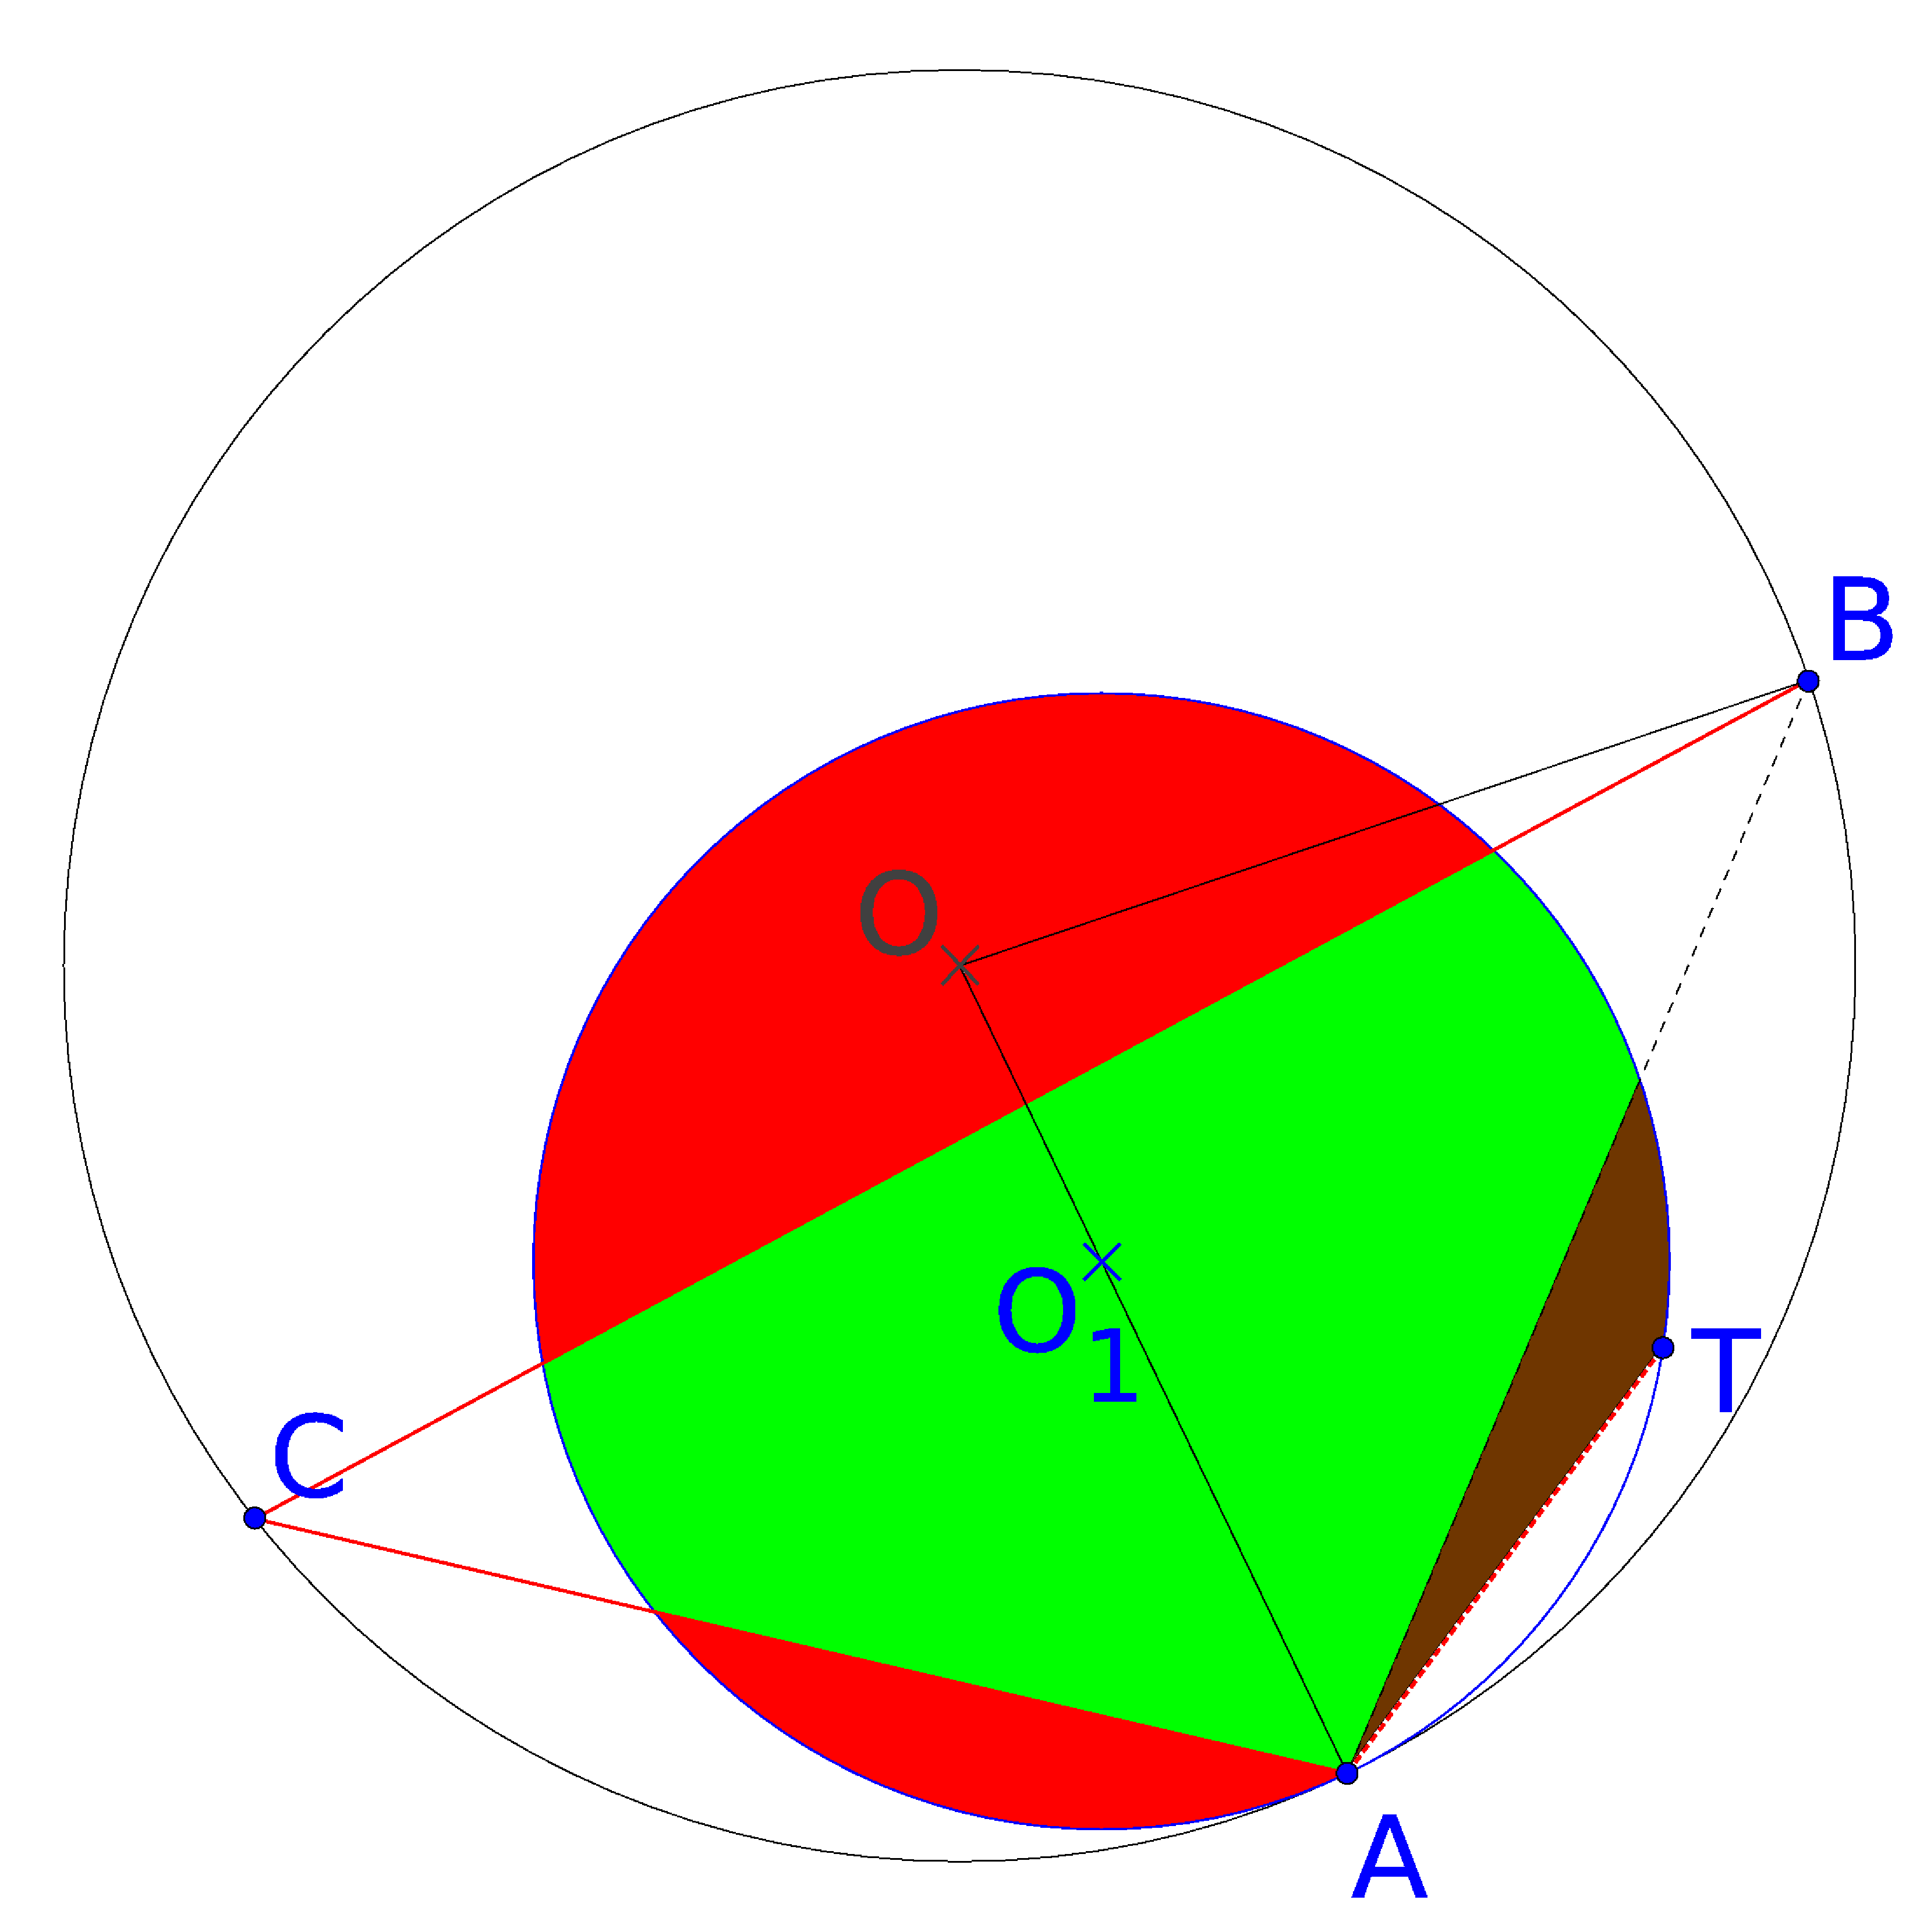
\includegraphics[width=0.5\linewidth]{eps/IntermediatePoint_beweis.eps}
%\caption{The red regions must be empty by lemma \ref{emptyregion}, the green area is empty by precondition and the brown region must be empty by ... }
%\label{fig:intermediate_point_beweis}
%\end{figure}
%
%
%\begin{enumerate}
%\item $|CA| + \sum\nolimits_{i=0}^{r-1} |M_iM_{i+1}| \leq (1+2\pi (k*\cos{\frac{\pi}{k}})^{-1})|CB| $
%\item There is no edge in G between any pair $M_i $ and $M_j $ lying in the closed region delimited by CA, CB and the edges of p, for any i and j satisfying $0 \leq i < j-1 \leq r $ 
%\item $\angle{M_{i-1}M_iM_{i+1}} > \frac{k-2}{k}\pi $, for $i=1, ..., r-1 $ 
%\item $\angle{CAM_1} \geq \frac{\pi}{2}-\frac{\pi}{k} $
%\end{enumerate}




\subsection{inward Path}
Now, we perform the proof for the case when $\triangle{ABC} $ contains other nodes.

Let $S $ be the set of points which contains points $A $ and $B $, and all the points interior to $\triangle{ABC} $ excluding $C $.
Then $CH(S) $ are all the points which are on the convex hull of $S $.
Let these points be called $N_0=A $ and $N_t=B $ and points $N_1 , \cdots ,N_{t-1} $ are the points on $CH(S) $ which lie inside $\triangle{ABC} $. 
The following proposition is taken from \cite{kanj}:
\begin{prop}
\label{inward_pre}
\begin{enumerate}
\renewcommand{\labelenumi}{\alph{enumi})}
The following are true:
\item for every $i =0,\cdots,s-1: $ $|CN_i| \leq |CN_{i+1}| $, and
\item for every $i=0, \cdots, s-2: $  $\angle{N_{i}N_{i+1}N_{i+2}} \geq \pi $, where $\angle{N_{i}N_{i+1}N_{i+2}} $ is the angle facing point $C $.
\end{enumerate} 
\end{prop}
\begin{proof}
Since $CA $ is the shortest edge in the angular sector $\angle{BCA} $, $|CA| \leq CN_i $, for $i=1 ,\cdots, t-1 $  and since $N_1 , \cdots, N_t $ are on $CH(S) $, a) is true.

Part b) follows from the convexity of $CH(S) $. All interior angles to $CH(S) $ measure at most $\pi $, so all the exterior angles fulfil $\angle{N_{i-1}N_iN_{i+1}}\geq \pi $ 
\end{proof}

Since $CN_i \leq CN_{i+1} $ and no other point of $G $ lies inside $\triangle{N_iCN_{i+1}} $, $CN_i $ is the shortest edge in the angular sector $\angle{N_iCN_{i+1}} $.
%related work: kanj hat neues ergebnis mit knotenbeschränkung kleiner gleich 11...
%improved local algorithms   2012
\section{Conclusion}
RMYS is due to its reactivity a robust algorithm to construct a bounded degree, planar graph which is most likely an Euclidean spanner.
As for now, it is not appropriate to use it to create a local view on just one node in consequence of the message overhead it creates.
However, it is well suited to create a complete graph in a reactive way while providing a constant node degree on top of planarity and a constant spanning ratio.
RMYS is the first algorithm which inherits all these graph properties and is created in a reactive way.

For the past years reactivity in ad hoc sensor networks reduced permanently the message overhead to create planar graphs which later turned out to be spanners.
In addition, it is now possible to append the property of a constant node degree for each node in the graph to reactive approaches.
This saves additional messages if a routing protocol uses the underlying RMYS graph.

In order to minimize the constant node degree bound of $14 $ further research should focus on formally proving the spanning ratio of RMYS and check whether it is possible to lower the degree bound without increasing the spanning ratio significantly.
Another interesting point for future research is to reduce the message overhead for RMYS when it is executed on one node.
For instance, under the condition that all possibilities where RMYS creates an uni directional edge are known (refer to figures \ref{fig:RMYS_case_one_cone_empty} and \ref{fig:RMYS_case_error_bidirectional} for help in this matter) one can possibly omit the last broadcast completely.
Instead, one must find a pattern for each of these possibilities to detect uni directional edges without sending additional messages.
\include{Programming}

%% LOT and LOF
\listoftables
\begingroup
\let\clearpage\relax
\listoffigures
\endgroup

\begin{appendix}
%% include your appendices here
%\include{appendix-A}
\end{appendix}
%%%%%%%%%%%%%%%%%%%%%%%%%%%%%%%%%%%%%%%%%%%%%%%%%%%%%%%%%%%%%%%%%
%%%%%%%%%%%%%%%%%%%%%%%%%%%%%%%%%%%%%%%%%%%%%%%%%%%%%%%%%%%%%%%%%
%\addcontentsline{toc}{chapter}{Bibliography}
\bibliographystyle{ieeetr}
{\footnotesize\bibliography{BachelorarbeitTim}}
\end{document}
%%%%%%%%%%%%%%%%%%%%%%%%%%%%%%%%%%%%%%%%%%%%%%%%%%%%%%%%%%%%%%%%%
%%%%%%%%%%%%%%%%%%%%%%%%%%%%%%%%%%%%%%%%%%%%%%%%%%%%%%%%%%%%%%%%%
\endinput
%%
%% End
